
% $Id: manual_tex.tex,v 1.2 2006-10-30 20:40:21 sarich Exp $ 
%
% LATEX version of the TAO users manual.
%
% manual_tex.tex is the base file for LaTeX format, while manual.tex is
% the corresponding base HTML format file.
%
\documentclass[11pt,openright]{book}
\usepackage{epsf}
\usepackage{amssymb}

% moreverb provides commands for reading and writing files. In particular,
% verbatiminput. See pages 66-70 on the LateX Companion.
\usepackage{moreverb}

% float supersedes the obsolete here package. See page 149 of the 
% LateX Companion.
\usepackage{float}

% url is a form of \verb intended for addresses, hypertext links, 
% directories/paths,...
\usepackage{url}
\usepackage{pdfpages}
\usepackage[bookmarksopen,colorlinks]{hyperref}

% afterpage places documents at the top of the page. See page 150 of the 
% LateX Companion.
\usepackage{afterpage}

\setlength{\textwidth}{6.0in}
\setlength{\oddsidemargin}{18pt}
\setlength{\evensidemargin}{18pt}
\setlength{\topmargin}{-0.5in}
\setlength{\textheight}{8.5in}

\newcommand{\half}{{\textstyle{\frac{1}{2}}}}
\newcommand{\findex}[1]{\index{#1}}
\newcommand{\sindex}[1]{\index{#1}}
\newcommand{\F}{\mbox{\boldmath \(F\)}}
\newcommand{\x}{\mbox{\boldmath \(x\)}}
\newcommand{\rr}{\mbox{\boldmath \(r\)}}
\newcommand{\R}{\mathbb R}
\renewcommand{\Re}{\R}
\newcommand{\Comment}[1]{}

\makeindex
 
% Defines the environment where design issues are discussed. In the manual
% version of this report, these regions are ignored.
\def\design{\medskip \noindent Design Issue:\begin{em}}
\def\enddesign{\end{em} \medskip}

% Print DRAFT in large letters across every page
%\special{!userdict begin /bop-hook{gsave 200 70 translate
%65 rotate /Times-Roman findfont 216 scalefont setfont
%0 0 moveto 0.95 setgray (DRAFT) show grestore}def end}

\begin{document}
\pagestyle {empty}


%\pagestyle {empty}
%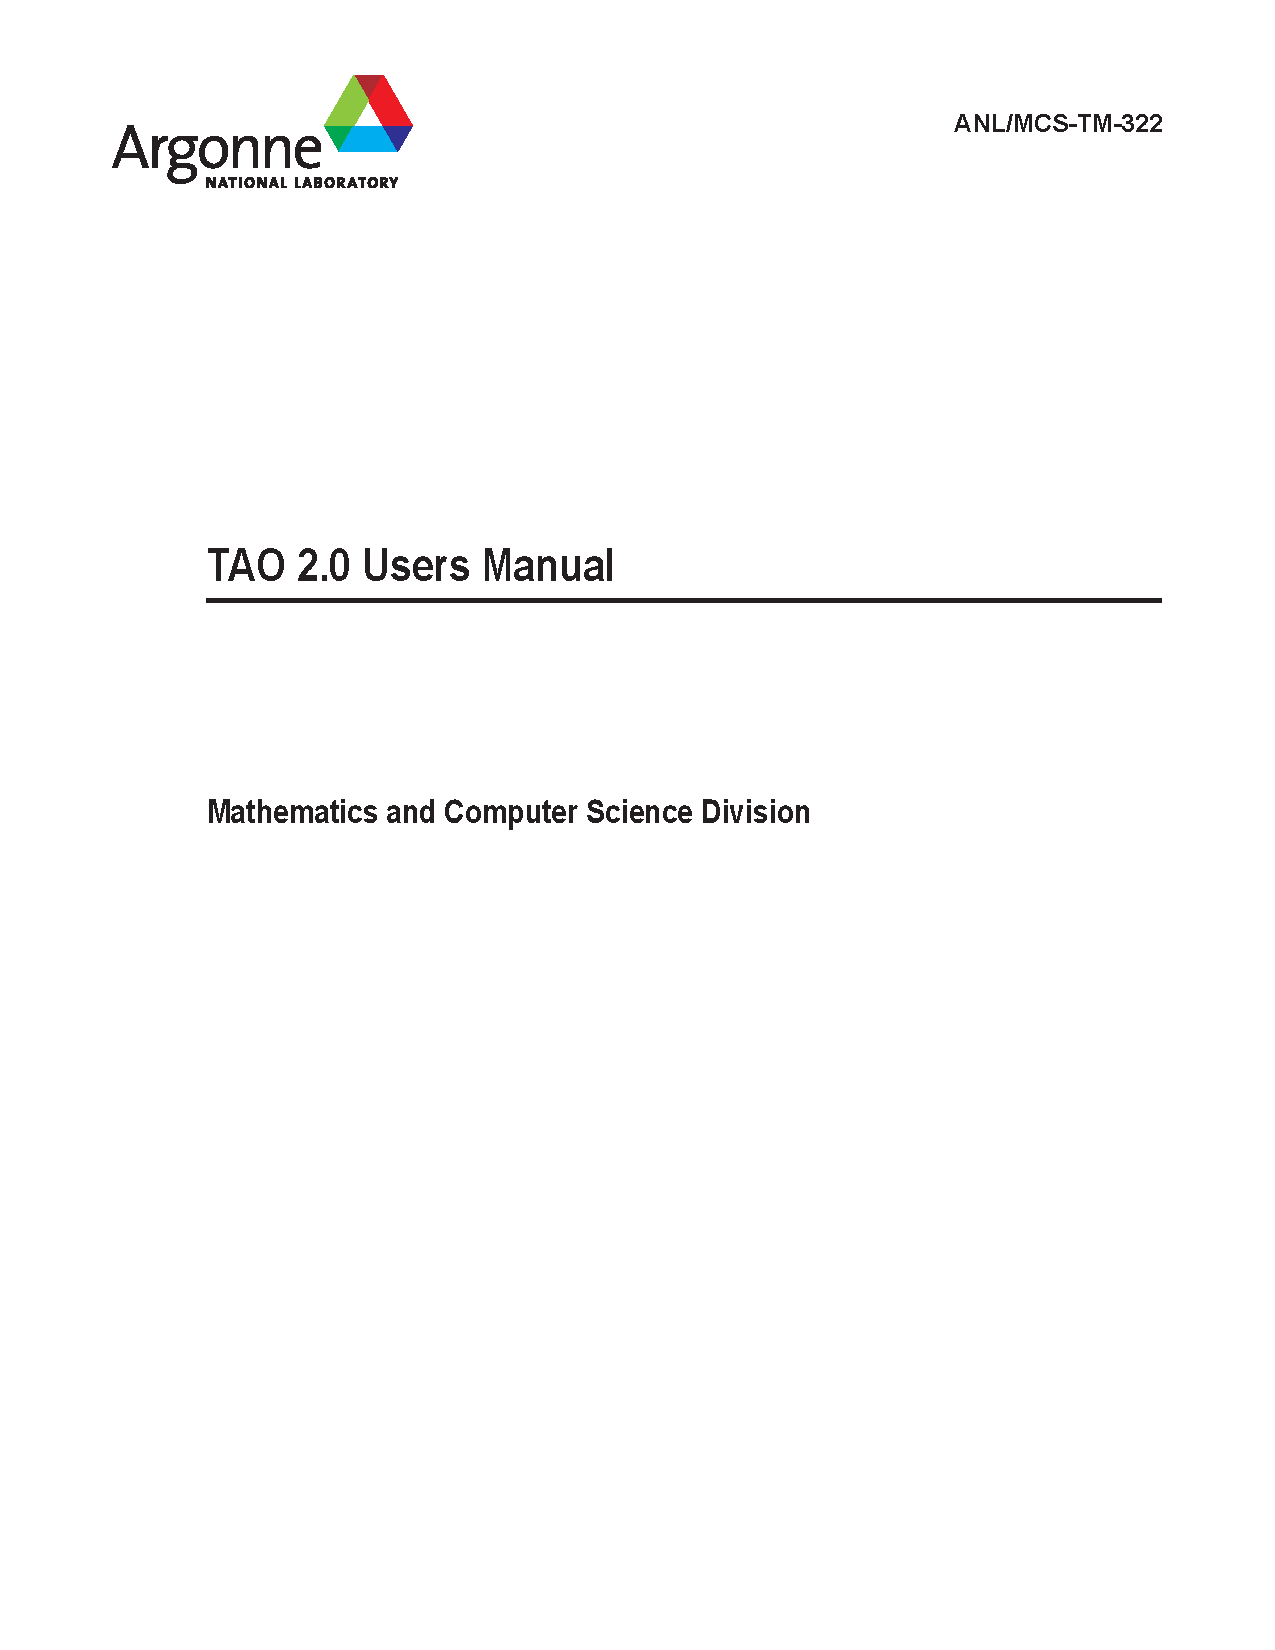
\includepdf[pages={1,2,3}]{ANL-MCS-TM-322.pdf}

\vspace{1.75in}

\begin{center}

ARGONNE NATIONAL LABORATORY

9700 South Cass Avenue

Argonne, Illinois  60439

\vspace{1.5in}

{\large
{\bf 
A CASE STUDY IN THE PERFORMANCE AND SCALABILITY OF
OPTIMIZATION ALGORITHMS
}
}

\vspace{.5in}

{\bf Steven J. Benson,
Lois Curfman McInnes, and
Jorge J. Mor\'e}

\vspace{.5in}

Mathematics and Computer Science Division

\vspace{.25in}

Preprint ANL/MCS-P768-0799

\vspace{.5in}

September 2000 (Revised May 2001)
\end{center}

\vspace{2.5in}

\bigskip


\par\noindent
This work was supported by the Mathematical, Information, and
Computational Sciences Division subprogram of the Office of Advanced
Scientific Computing, U.S. Department of Energy, under Contract
W-31-109-Eng-38.


% Table of contents.
\cleardoublepage
\pagestyle {plain}
\pagenumbering{roman}
\setcounter{page}{1}
\tableofcontents

\cleardoublepage
% Abstract for TAO Users Manual

\addcontentsline{toc}{chapter}{Preface}
\section*{Preface}

The Toolkit for Advanced Optimization (TAO) focuses on the development
of algorithms and software for the solution of large-scale optimization 
problems on high-performance architectures.  Areas of interest include 
unconstrained and bound-constrained optimization, nonlinear least squares 
problems, optimization problems with partial differential equation 
constraints, and variational inequalities and complementarity 
constraints.

The development of TAO was motivated by the scattered support for
parallel computations and the lack of reuse of external toolkits in
current optimization software.  Our aim is to produce high-quality 
optimization software for computing environments ranging from 
workstations and laptops to massively parallel high-performance 
architectures.  Our design decisions are strongly motivated by 
the challenges inherent in the use of large-scale distributed 
memory architectures and the reality of working with large, 
often poorly structured legacy codes for specific 
applications.

%%% Local Variables: 
%%% mode: latex
%%% TeX-master: "manual_tex"
%%% End: 



\addcontentsline{toc}{chapter}{Changes for Version 3.5}
\section*{Changes in Version 3.5}
TAO is now included in the PETSc distribution and the PETSc
repository, thus it versions will always match the PETSc version. The
TaoSolver object is now simply Tao and there is no TaoInitialize() or
TaoFinalize(). Numerious changes have been made to make the source
code more PETSc-like.  All future changes will be listed in the PETSc changes documentation.

\addcontentsline{toc}{chapter}{Changes for Version 2.0}
\section*{Changes in Version 2.0}

TAO version numbers will now adhere to the new PETSc standard of 
Major-Minor-Patch. Any patch-level changes will have an attempt to keep the 
applicatin programming interface (API) untouched, but in any case backward 
compatibility with previous version of the minor version will be 
maintained.

Many new features and interface changes were introduced in TAO version 2.0 (and continue to be used in version 2.2.0).
TAO applications created for previous versions will need to be updated to 
work with the new version.  We apologize for any inconvenience this situation
may cause; these changes were needed to keep the interface
clean, 
clear, and easy to use. Some of the most important changes are highlighted 
below.

\vspace{7mm}
\noindent \textbf{Elimination of the TaoApplication Object}. The largest change to the TAO programming interface was the elimination of the
TaoApplication data structure. In previous versions of TAO, this structure was 
created by the application programmer for application-specific data and 
routines.  In order to more closely follow PETSc design principles, this 
information is now directly attached to a Tao object instead.  See 
Figure~\ref{fig:tao_commands} for a listing of what the most common TAO 
routines now look like without the TaoApplication object.

\vspace{7mm}
\noindent \textbf{New Algorithms}. TAO has a new algorithm for solving derivative-free nonlinear least
squares
problems, POUNDerS, that can efficiently solve parameter optimization problems 
when no derivatives are available and function evaluations are expensive. 
See 
Section~\ref{sec:pounders} for more information on the details of the 
algorithm and Section~\ref{sec:leastsquares} for how to use it.
TAO now also provides a new algorithm for the solution of optimization
problems with partial differential equation (PDE) constraints based on a
linearly constrained augmented Lagrangian (LCL) method.  More 
information on PDE-constrained optimization and LCL can be found 
in Section~\ref{sec:lcl}.


\vspace{7mm}
\noindent \textbf{TaoLineSearch Object}. TAO has promoted the line search to a full object.  Any of the available 
TAO line search algorithms (Armijo, Mor\'e-Thuente, GPCG, and unit) can now 
be selected regardless of the overlying TAO algorithm.  Users can also
create new line search algorithms that may be more suitable for their
applications.  More information is available in 
Section~\ref{sec:TaoLineSearch}.

\vspace{7mm}
\noindent \textbf{Better Adherence to PETSc Style}. TAO now features a tighter association with PETSc standards and practices.  All 
TAO constructs now follow PETSc conventions and are written in C.  There is 
no longer a separate abstract class for vectors, matrices, and linear 
solvers. TAO now uses these PETSc objects directly.  We believe these 
changes make TAO applications much easier to create and maintain for 
users already familiar with PETSc programming. These changes also allow 
TAO to relax some of the previously imposed requirements on the PETSc 
configuration.  TAO now works with PETSc configured with single-precision 
and quad-precision arithmetic when using GNU compilers and no longer 
requires a C++ compiler.  However, TAO is not compatible with PETSc 
installations using complex data types.



% Acknowledgements for PETSc Users Manual
%
%   this information is a DUPLICATE of misc/acknwldg.htm
%                MAKE SURE THEY MATCH!!!
%
\noindent {\bf Acknowledgments:}

\medskip \medskip \noindent
We thank all PETSc users for their many suggestions, bug reports, and
encouragement.  We especially thank David Keyes
for his valuable comments on the source code,
functionality, and documentation for PETSc.


\vspace{.3in}
\noindent
Some of the source code and utilities in PETSc
have been written by
\begin{itemize}
  \item Asbjorn Hoiland Aarrestad - the explicit Runge-Kutta implementations;
  \item G. Anciaux and J. Roman - the interfaces to the partitioning packages PTScotch, Chaco, and Party;
  \item Allison Baker - the flexible GMRES code and LGMRES;
  \item Chad Carroll - Win32 graphics;
  \item Ethan Coon - the PetscBag and many bug fixes;
  \item Cameron Cooper - portions of the VecScatter routines;
  \item Patrick Farrell - nleqerr line search for SNES
  \item Paulo Goldfeld - balancing Neumann-Neumann preconditioner;
  \item Matt Hille;
  \item Joel Malard - the BICGStab(l) implementation;
  \item Paul Mullowney, enhancements to portions of the Nvidia GPU interface;
  \item Dave May - the GCR implementation
  \item Peter Mell - portions of the DA routines;
  \item Richard Mills - the AIJPERM matrix format for the Cray X1 and universal F90 array interface;
  \item Victor Minden - the NVidia GPU interface;
  \item Todd Munson - the LUSOL (sparse solver in MINOS) interface and several Krylov methods;
  \item Adam Powell - the PETSc Debian package,
  \item Robert Scheichl - the MINRES implementation,
  \item Kerry Stevens - the pthread based Vec and Mat classes plus the various thread pools
  \item Karen Toonen - designed and implemented much of the PETSc web pages,
  \item Desire Nuentsa Wakam - the deflated GMRES implementation,
  \item Liyang Xu - the interface to PVODE (now Sundials/CVODE).
\end{itemize}

\vspace{.3in}
\noindent
PETSc source code contains modfied routines from the following public domain software packages
\begin{itemize}
  \item LINPACK -    dense matrix factorization and solve; converted to C using {\tt f2c} and then
                     hand-optimized for small matrix sizes, for block matrix data structures;
  \item MINPACK -    see page \pageref{sec_fdmatrix}, sequential matrix coloring routines for finite difference Jacobian
                     evaluations; converted to C using {\tt f2c};
  \item SPARSPAK -   see page \pageref{sec_factorization}, matrix reordering routines, converted to C using {\tt f2c};
  \item libtfs     - the efficient, parallel direct solver developed by Henry Tufo and Paul Fischer for the direct solution of a coarse grid problem
                     (a linear system with very few degrees of freedom per processor).
\end{itemize}


\vspace{.3in}
\noindent
PETSc interfaces to the following external software:
\begin{itemize}
  \item ADIFOR -  automatic differentiation for the computation of sparse Jacobians,\\
                     \href{http://www.mcs.anl.gov/adifor}{http://www.mcs.anl.gov/adifor},
  \item BLAS and LAPACK - numerical linear algebra,
  \item Chaco -     A graph partitioning package, \href{ http://www.cs.sandia.gov/CRF/chac.html}{ http://www.cs.sandia.gov/CRF/chac.html}
  \item ESSL -         IBM's math library for fast sparse direct LU factorization,
  \item Elemental -  Jack Poulson's parallel dense matrix solver package,
  \item hypre -    the LLNL preconditioner library, \href{http://www.llnl.gov/CASC/hypre}{http://www.llnl.gov/CASC/hypre}
  \item LUSOL -       sparse LU factorization code (part of MINOS) developed by Michael Saunders,
                      Systems Optimization Laboratory, Stanford University,
                     \href{http://www.sbsi-sol-optimize.com/}{http://www.sbsi-sol-optimize.com/},
  \item Mathematica -  see page \pageref{ch_mathematica},
  \item MATLAB -      see page \pageref{ch_matlab},
  \item MUMPS -      see page \pageref{sec_externalsol}, MUltifrontal Massively Parallel sparse direct Solver developed by Patrick Amestoy,
                     Iain Duff, Jacko Koster, and Jean-Yves L'Excellent, \\
                     \href{http://www.enseeiht.fr/lima/apo/MUMPS/credits.html}{http://www.enseeiht.fr/lima/apo/MUMPS/credits.html},
  \item Metis/ParMeTiS - see page \pageref{sec_partitioning}, parallel graph partitioner,
                     \href{http://www-users.cs.umn.edu/~karypis/metis/}{http://www-users.cs.umn.edu/~karypis/metis/},
  \item Party -     A graph partitioning package, \\ 
               \href{http://www2.cs.uni-paderborn.de/cs/ag-monien/PERSONAL/ROBSY/party.html}{http://www2.cs.uni-paderborn.de/cs/ag-monien/PERSONAL/ROBSY/party.html},
  \item PaStiX -     Parallel LU and Cholesky solvers,
  \item PTScotch -    A graph partitioning package, \href{http://www.labri.fr/Perso/~pelegrin/scotch/}{http://www.labri.fr/Perso/~pelegrin/scotch/}
  \item SPAI -        for parallel sparse approximate inverse preconditiong,
  \item SparseSuite - see page \pageref{sec_externalsol},  developed by Timothy A. Davis,
                    \href{http://faculty.cse.tamu.edu/davis/suitesparse.html}{http://faculty.cse.tamu.edu/davis/suitesparse.html}.
  \item Sundial/CVODE - see page \pageref{sec_sundials}, parallel ODE integrator,
                     \href{http://www.llnl.gov/CASC/sundials/}{http://www.llnl.gov/CASC/sundials/},
  \item SuperLU and SuperLU\_Dist - see page \pageref{sec_externalsol},
                    the efficient sparse LU codes developed by Jim Demmel,  Xiaoye S. Li, and John Gilbert,
                    \href{http://crd-legacy.lbl.gov/~xiaoye/SuperLU}{http://crd-legacy.lbl.gov/~xiaoye/SuperLU},
  \item Triangle and Tetgen - mesh generation packages,
  \item Trilinos/ML - Sandia's main multigrid preconditioning package, \href{http://software.sandia.gov/trilinos/}{http://software.sandia.gov/trilinos/},
  \item Zoltan - graph partitioners from Sandia National Laboratory
\end{itemize}
These are all optional packages and do not need to be installed to use PETSc.

PETSc software is developed and maintained using
\begin{itemize}
\item Emacs editor
\item \href{http://git-scm.com/}{Git} revision control system
\item Python
\end{itemize}

PETSc documentation has been generated using
\begin{itemize}
\item the \href{http://www.cs.uiuc.edu/~wgropp/projects/software/sowing/index.htm}{text processing tools} developed by Bill Gropp
\item c2html
\item pdflatex
\item python
\end{itemize}



\cleardoublepage
\addcontentsline{toc}{chapter}{License}
\noindent
Copyright © 2013, UChicago Argonne, LLC \\
Operator of Argonne National Laboratory \\
All rights reserved. \\
Toolkit for Advanced Optimization (TAO), Version 2.2.0 \\
OPEN SOURCE LICENSE \\

\noindent
Redistribution and use in source and binary forms, with or without modification, are permitted provided that the following conditions are met:
\begin{itemize}
\item    Redistributions of source code must retain the above copyright notice, this list of conditions and the following disclaimer. Software changes, modifications, or derivative works, should be noted with comments and the author and organization's name. \\
\item    Redistributions in binary form must reproduce the above copyright notice, this list of conditions and the following disclaimer in the documentation and/or other materials provided with the distribution. \\
\item    Neither the names of UChicago Argonne, LLC nor the Department of Energy nor the names of its contributors may be used to endorse or promote products derived from this software without specific prior written permission. \\
\item    The software and the end-user documentation included with the redistribution, if any, must include the following acknowledgment:\\
    ``This product includes software produced by UChicago Argonne, LLC under Contract No. DE-AC02-06CH11357 with the Department of Energy.''
\end{itemize}

\noindent
********************************************************************************\\
\noindent
DISCLAIMER \\

\noindent
THE SOFTWARE IS SUPPLIED ``AS IS'' WITHOUT WARRANTY OF ANY KIND.\\
NEITHER THE UNITED STATES GOVERNMENT, NOR THE UNITED STATES\\
DEPARTMENT OF ENERGY, NOR UCHICAGO ARGONNE, LLC, NOR ANY OF\\
THEIR EMPLOYEES, MAKES ANY WARRANTY, EXPRESS OR IMPLIED, OR\\
ASSUMES ANY LEGAL LIABILITY OR RESPONSIBILITY FOR THE ACCURACY,\\
COMPLETENESS, OR USEFULNESS OF ANY INFORMATION, DATA,\\
APPARATUS, PRODUCT, OR PROCESS DISCLOSED, OR REPRESENTS THAT\\
ITS USE WOULD NOT INFRINGE PRIVATELY OWNED RIGHTS.\\

\noindent
********************************************************************************\\


% Start of the Users Manual
\cleardoublepage
\setcounter {page}{1}
\pagenumbering{arabic}

\chapter{Introduction}
\label{chapter:introduction}

% Very introductory, gentle introduction. Pretty tables and figures.
% Perhaps use preamble of \ref{chapter:Getting Started}
% Written in C, but good with C++ compilers.  Also can use fortran.

The Toolkit for Advanced Optimization (TAO) focuses on the design and
implementation of optimization software for 
solving large-scale optimization applications on high-performance
architectures.  Our approach is motivated by the scattered support for
parallel computations and lack of reuse of linear algebra software in
currently available optimization software.  The TAO design allows the
reuse of toolkits that provide lower-level support (parallel sparse
matrix data structures, preconditioners, solvers), and thus we are
able to build on top of these toolkits instead of having to redevelop
code. The advantages in terms of efficiency and development time are
significant.  This chapter provides a short introduction to our design 
philosophy and the importance of this design.

% The TAO design philosophy uses object-oriented techniques of data and
% state encapsulation, abstract classes, and limited inheritance to
% create a flexible optimization toolkit.  

%Use MPI, Microkernal 
% Goals, Current state of art. AD support
%\section{} Use matrices, vectors, linear solvers, as TAO objects

The TAO design philosophy place strong emphasis on the reuse of
external tools where appropriate.  Our design enables bidirectional
connection to lower-level linear algebra support (e.g., parallel sparse
matrix data structures) provided in toolkits such as PETSc
\cite{petsc-web-page,petsc,petsc-user-ref}
vas well as higher-level application
frameworks.  Our design decisions are strongly motivated by the
challenges inherent in the use of large-scale distributed memory
architectures and the reality of working with large and often poorly
structured legacy codes for specific applications.  Figure
\ref{tao:design} illustrates how the TAO software works with external
libraries and application code.

\begin{figure}[ht]
\centering{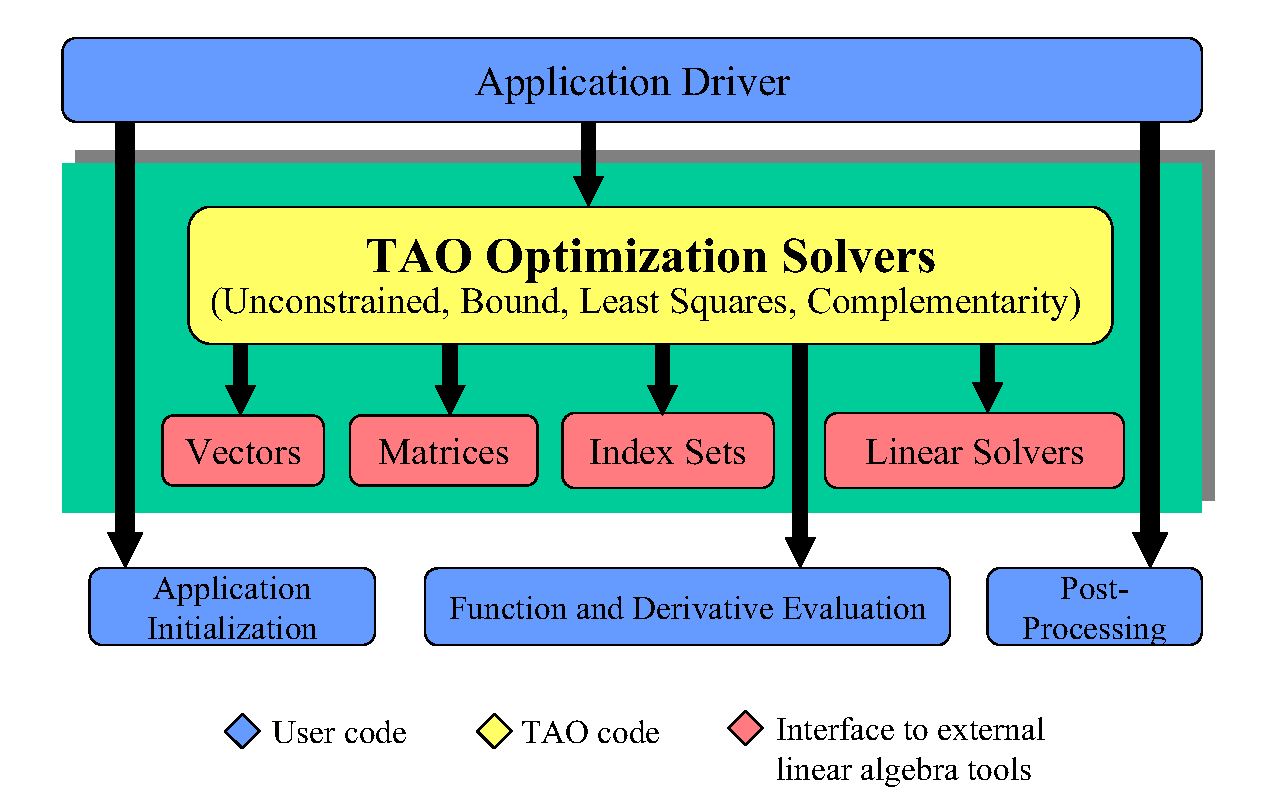
\includegraphics[height=3.5in,clip]{taofig.pdf}}
\caption{TAO Design}
\label{tao:design}
\end{figure}

%\begin{figure}
%\centerline{\epsfysize=3.5in \epsfbox{taofig.eps}}
%\caption{TAO Design}
%\label{tao:design}
%\end{figure}


The TAO solvers use fundamental PETSc objects to define and solve
optimization problems: vectors, matrices, index sets, and linear
solvers.  The concepts of vectors and matrices are standard, while an
index set refers to a set of integers used to identify particular
elements of vectors or matrices.  An optimization algorithm is a
sequence of well-defined operations on these objects.  These
operations include vector sums, inner products, and matrix-vector
multiplication.

With sufficiently flexible abstract interfaces, PETSc can support a
variety of implementations of data structures and algorithms.  These
abstractions allow us to more easily experiment with a range of
algorithmic and data structure options for realistic problems.  
Such capabilities are critical for making
high-performance optimization software adaptable to the continual
evolution of parallel and distributed architectures and the research
community's discovery of new algorithms that exploit their features.

\begin{comment}
The TAO design philosophy eliminates some of the barriers in using
independently developed software components by accepting data that is
independent of representation and calling sequence written for
particular data formats.  Our current TAO implementation uses 
the parallel system infrastructure and linear algebra objects 
offered by PETSc version 3.3, which uses MPI \cite{using-mpi} 
for all interprocessor communication.  The PETSc package supports 
objects for vectors, matrices, index sets, and linear solvers
using various formats and has links to external linear algebra
\section{Performance Results}

A major concern in the TAO project is the performance and scalability
of optimization algorithms on large problems.  In this section we
focus on the GPCG (gradient projection, conjugate gradient) algorithm
for the solution of bound-constrained convex quadratic programming
problems.  Originally developed by Mor\'e and Toraldo
\cite{more-toraldo}, the GPCG algorithm was designed for large-scale
problems but had only been implemented for a single processor.  GPCG
combines the advantages of the identification properties of the
gradient projection method with the finite termination properties of
the conjugate gradient method.  Moreover, the performance of the
TAO implementation on large optimization problems is noteworthy.

%\begin{figure}[tb]
%\centering{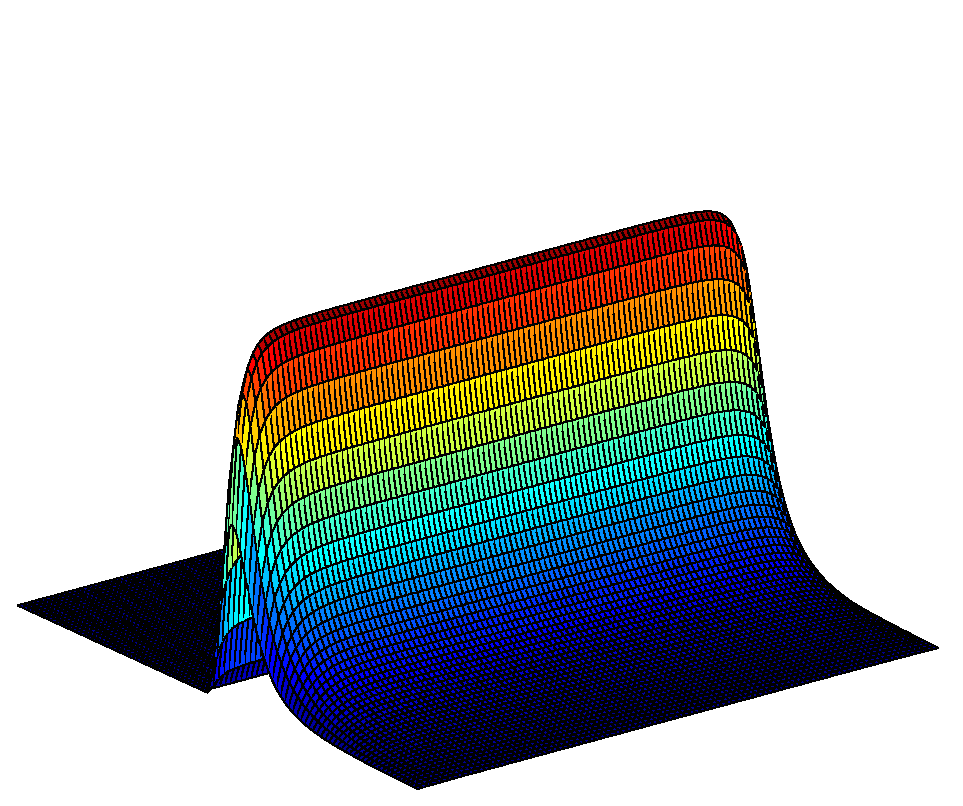
\includegraphics[height=3.0in]{pjb.eps}}
%\caption{The journal bearing problem with $\epsilon$ = 0.9}
%\label{dpjb}
%\end{figure}

\begin{figure}[tb]
\centerline{\epsfysize=3.0in \epsfbox{pjb.eps}}
\caption{The journal bearing problem with $\epsilon$ = 0.9}
\label{dpjb}
\end{figure}



We illustrate the performance of the GPCG algorithm by 
presenting results for a journal bearing problem
with over 2.5 million variables.
The journal bearing problem
is a finite element approximation to a variational problem 
over a rectangular two-dimensional grid.  A
grid with $1600$ points in each direction, for example, is formulated
as a bound-constrained quadratic problem with $1600^2=2,560,000$
variables.
The triangulation of the grid results in a matrix that has the
usual five diagonal nonzero structure that arises
from a difference approximation to the Laplacian operator.
The journal bearing problem contains an eccentricity parameter,
$\varepsilon \in (0,1)$, that influences the number of active
variables at the solution and the difficulty in solving it.
Figure \ref{dpjb} shows the solution of the journal bearing problem
for $ \varepsilon = 0.9 $. The steep gradient in the solution
makes this problem a difficult benchmark.

The performance results in Table \ref{flops} are noteworthy is several
ways.  First of all, the number of faces visited by GPCG is remarkably
small.  Other strategies can lead to a large number of gradient
projection iterates, but the GPCG algorithm is remarkably efficient.
Another interesting aspect of these results is that due to the low
memory requirements of iterative solvers, we were able to solve these
problems with only $ p = 8 $ processors.  Strategies that rely on
direct solvers are likely to need significantly more storage, and thus
more processors.  Finally, these results show that the GPCG
implementation has excellent efficiency.  For example, the efficiency
of GPCG with respect to $ p = 8 $ processors ranges between $ 70\% $
and $ 100\% $ when $ \varepsilon = 0.1 $.  This sustained efficiency
is remarkable since the GPCG algorithm is solving a sequence of linear
problems with a coefficient matrix set to the submatrix of the Hessian
matrix with respect to the free variables for the current iterate.
Thus, our implementation's repartitioning of submatrices effectively
deals with the load-balancing problem that is inherent in the GPCG
algorithm.

\begin{table}[htb]
\begin{center}
\begin{tabular}{| c r | c c r c r |}
\hline
\multicolumn{1}{|c}{$ \varepsilon $} & 
\multicolumn{1}{c|}{$ p $} & 
\multicolumn{1}{c}{faces} &
\multicolumn{1}{c}{$n_{CG}$} & 
\multicolumn{1}{c}{time} &
\multicolumn{1}{c}{$t_{CG}$\%} & 
\multicolumn{1}{c|}{$ \cal E $} \\ \hline
0.1  & 8 & 46 & 431 & 7419 & 86 & 100  \\ 
0.1  & 16 & 45 & 423 & 3706 & 83 & 100  \\
0.1  & 32 & 45 & 427 & 2045 & 82 & 91 \\
0.1  & 64 & 45 & 427 & 1279 & 82 & 73 \\
\hline
0.9  & 8 & 37 & 105 & 2134 & 70 & 100 \\
0.9  & 16 & 37 & 103 & 1124 & 71 & 95 \\
0.9  & 32 & 38 & 100 & 618 & 69 & 86 \\
0.9  & 64 & 38 & 99 & 397 & 68 & 67 \\
\hline
\end{tabular}
\caption{Performance of GPCG on the journal bearing problem
with $ 2.56 \cdot 10^6 $ variables.}
\label{flops}
\end{center}
\end{table}




An important aspect of our results that is not
apparent from Table \ref{flops} is that 
for these results we were able to experiment easily 
with all the preconditioners offered by PETSc.
In particular, we were able to compare the diagonal Jacobi
preconditioner with block Jacobi and overlapping additive Schwarz
preconditioners that use a zero-fill ILU solver in each block.  We
also experimented with a parallel zero-fill incomplete Cholesky preconditioner
provided by a PETSc interface to the BlockSolve95~\cite{bs-user-ref}
package of Jones and
Plassmann.  Interestingly enough, the diagonal Jacobi preconditioner
achieved better performance on this problem.



%%% Local Variables: 
%%% mode: latex
%%% TeX-master: "manual_tex"
%%% End: 
\end{comment}


% --------------------------------------------------------------------
%
%                            PART 1
%
%   This introductory PETSc information is included in
%   both manual.tex and intro.tex.
%
% --------------------------------------------------------------------

\label{sec_gettingstarted}

The Portable, Extensible Toolkit for Scientific Computation (PETSc)
has successfully demonstrated that the use of modern programming
paradigms can ease the development of large-scale scientific
application codes in Fortran, C, C++, and Python.  Begun several years ago,
the software has evolved into a powerful set of tools for the
numerical solution of partial differential equations and related problems
on high-performance computers. 

PETSc consists of a variety of libraries (similar to classes in C++),
which are discussed in detail in Parts II and III of the users manual.
Each library manipulates a particular family of objects (for instance,
vectors) and the operations one would like to perform on the objects.
The objects and operations in PETSc are derived from our long
experiences with scientific computation. Some of the PETSc modules deal with
\begin{itemize}
\item index sets (IS), including permutations, for indexing into vectors, renumbering, etc;
\item vectors (Vec);
\item matrices (Mat) (generally sparse);
\item managing interactions between mesh data structures and vectors and matrices (DM);
\item over fifteen Krylov subspace methods (KSP);
\item dozens of preconditioners, including multigrid, block solvers, and sparse direct solvers (PC);
\item nonlinear solvers (SNES); and
\item timesteppers for solving time-dependent (nonlinear) PDEs, including support for differential algebraic equations (TS).
\end{itemize}
Each consists of an abstract interface
(simply a set of calling sequences) and one or more implementations
using particular data structures. Thus, PETSc provides clean and
effective codes for the various phases of solving PDEs, with a uniform
approach for each class of problems.  This design
enables easy comparison and use of different algorithms (for example,
to experiment with different Krylov subspace methods, preconditioners,
or truncated Newton methods).
Hence, PETSc provides a rich environment for modeling scientific
applications as well as for rapid algorithm design and prototyping.

The libraries enable easy customization and extension of both algorithms
and implementations.  This approach promotes code reuse and
flexibility, and separates the issues of parallelism from the choice
of algorithms.  The PETSc infrastructure creates a
foundation for building large-scale applications.

It is useful to consider the interrelationships among different
pieces of PETSc.  Figure \ref{fig_1} is a diagram of some
of these pieces; Figure \ref{fig_2} presents
several of the individual parts in more detail.
These figures illustrate the library's hierarchical organization,
which enables users to employ the level of abstraction that is most
appropriate for a particular problem.
\begin{figure}[hbt]
%\centerline{ \pdfximage height 3.4in {petscwww.pdf} \pdfrefximage \pdflastximage}
\centerline{ 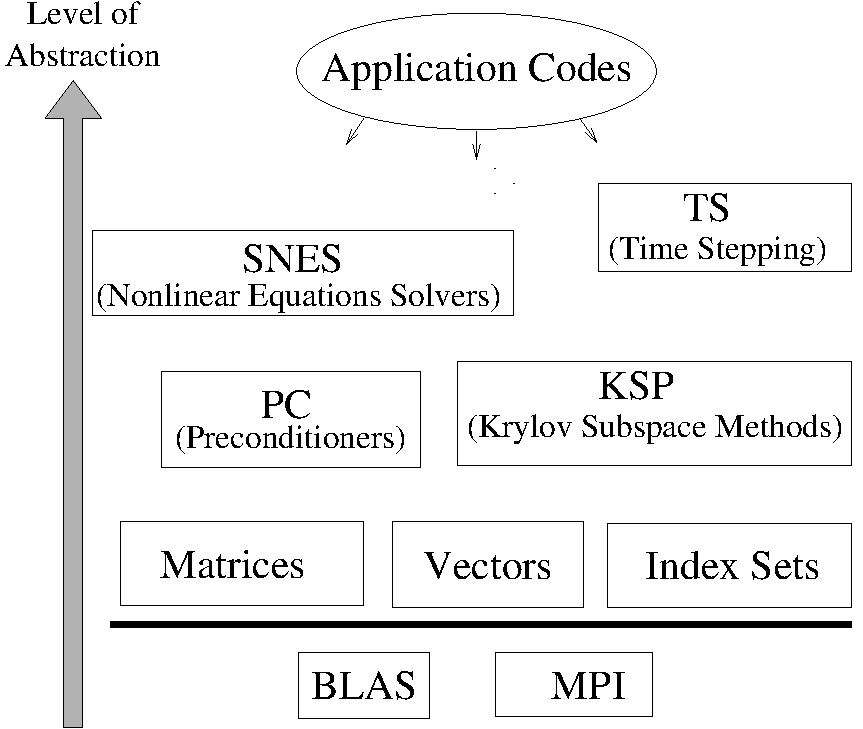
\includegraphics{petscwww}}
%\centerline{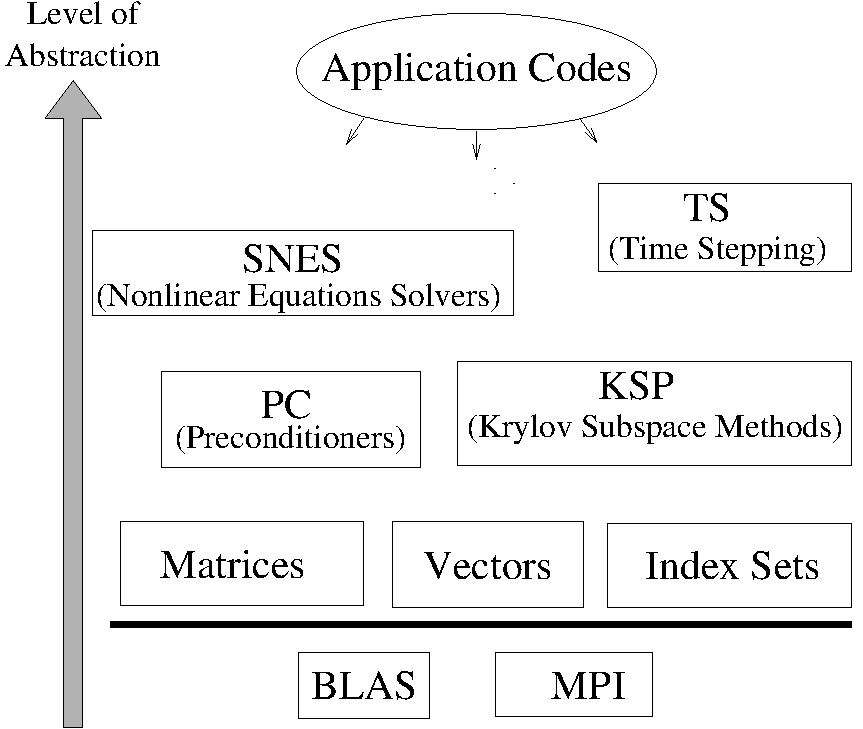
\psfig{file=petscwww.ps,angle=270,height=3.4in}}
% \centerline{\psfig{file=petsc_pt.eps,angle=0,height=4in,width=5in}}
\caption{Organization of the PETSc Libraries}
\label{fig_1}
\end{figure}

\begin{figure}[hbt]
\centerline{ 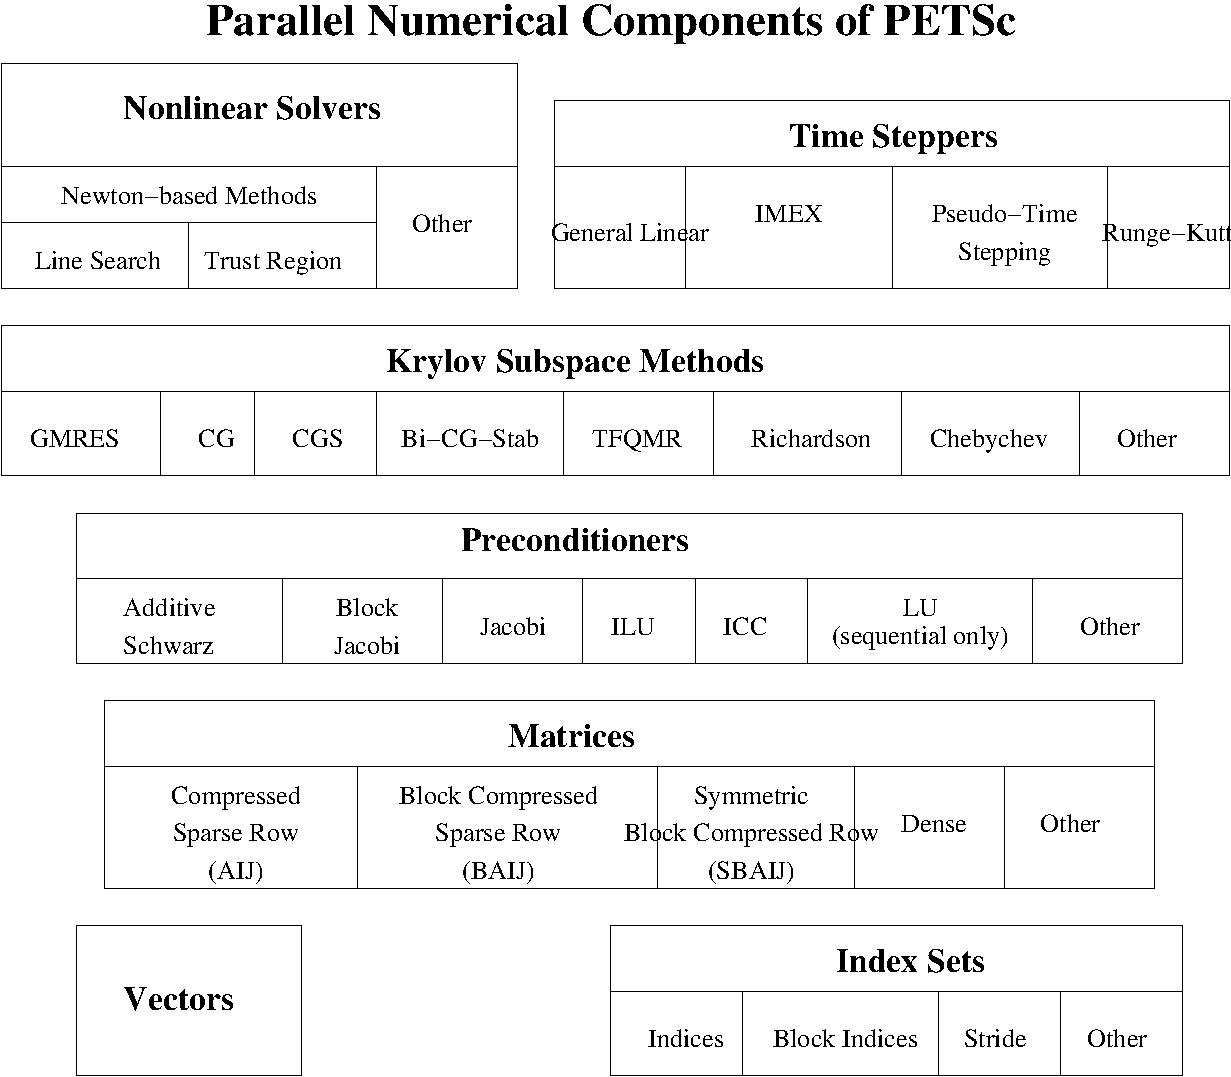
\includegraphics[scale=0.75]{zoom}}
%\centerline{\psfig{file=zoom_ls.ps,angle=270,height=3.4in}}
\caption{Numerical Libraries of PETSc}
\label{fig_2}
\end{figure}

\section{Suggested Reading}

The manual is
divided into three parts:
\begin{itemize}
\item Part I - Introduction to PETSc
\item Part II - Programming with PETSc
\item Part III - Additional Information
\end{itemize}

Part I describes
the basic procedure for using the PETSc library and presents two
simple examples of solving linear systems with PETSc.  This section
conveys the typical style used throughout the library and enables the
application programmer to begin using the software immediately.
Part I is also distributed separately for individuals interested in an
overview of the PETSc software, excluding the details of library usage.
Readers of this separate distribution of Part I should note that all
references within the text to particular chapters and sections
indicate locations in the complete users manual.

Part II explains in detail the use of the various PETSc libraries,
such as vectors, matrices, index sets, linear and nonlinear
solvers, and graphics.  Part III describes a variety of useful
information, including profiling, the options database, viewers, error
handling, makefiles, and some details of
PETSc design.

\nocite{efficient}

PETSc has evolved to become quite a comprehensive package, and therefore the
{\em PETSc Users Manual} can be rather intimidating for new users. We
recommend that one initially reads the entire document before proceeding with
serious use of PETSc, but bear in mind that PETSc can be used efficiently
before one understands all of the material presented here. Furthermore, the
definitive reference for any PETSc function is always the online manualpage.

\medskip \medskip

Within the PETSc distribution, the directory \trl{${PETSC_DIR}/docs}
contains all documentation.
Manual pages for all PETSc functions can be
accessed at \href{http://www.mcs.anl.gov/petsc/documentation}{http://www.mcs.anl.gov/petsc/documentation}.
The manual pages
provide hyperlinked indices (organized by
both concepts and routine names) to the tutorial examples and enable
easy movement among related topics.

Emacs and Vi/Vim users may find the
\trl{etags}/\trl{ctags}  option to be extremely useful for exploring the PETSc
source code.  Details of this feature are provided in
Section~\ref{sec_emacs}.

The file \trl{manual.pdf} contains
the complete {\em PETSc Users Manual} in the portable document format (PDF),
while \trl{intro.pdf}
includes only the introductory segment, Part I.  \sindex{installing PETSc}
The complete PETSc distribution, users
manual, manual pages, and additional information are also available via
the PETSc home page at
\href{http://www.mcs.anl.gov/petsc}{http://www.mcs.anl.gov/petsc}.
The PETSc home page also
contains details regarding installation, new features and changes in recent
versions of PETSc, machines that we currently support, and a FAQ list for frequently asked questions.

\medskip\medskip

\noindent{\bf Note to Fortran Programmers}: In most of the
manual, the examples and calling sequences are given for the C/C++
family of programming languages.  We follow this convention because we
recommend that PETSc applications be coded in C or C++.
However, pure Fortran programmers can use most of the
functionality of PETSc from Fortran, with only minor differences in
the user interface.  Chapter \ref{ch_fortran} provides a discussion of the
differences between using PETSc from Fortran and C, as well as several
complete Fortran examples.  This chapter also introduces some
routines that support direct use of Fortran90 pointers.

\noindent{\bf Note to Python Programmers}: To program with PETSc in Python you need to install the PETSc4py package developed by
Lisandro Dalcin. This can be done by configuring PETSc with the option \trl{--download-petsc4py}. See the PETSc installation guide
for more details \href{http://www.mcs.anl.gov/petsc/documentation/installation.html}{http://www.mcs.anl.gov/petsc/documentation/installation.html}.

\noindent{\bf Note to MATLAB Programmers}: The code that allows PETSc to be called from MATLAB is not currently supported due to the lack of interest and use.
If you are very interested in using and and taking over its
maintenance please contact us. To program with PETSc in MATLAB read the information in
share/petsc/matlab/classes/PetscInitialize.m. Numerous examples are
given in share/petsc/matlab/classes/examples/tutorials. Run the
program demo in that directory.

%-----------------------------------------------------------------------------
\section{Running PETSc Programs}
\label{sec_running}

Before using PETSc, the user must first set the environmental variable
\trl{PETSC_DIR}, \findex{PETSC_DIR} indicating the full path of the PETSc home
directory.  For example, under the UNIX bash shell a command of the form
\begin{tabbing}
   export PETSC\_DIR=\$HOME/petsc
\end{tabbing}
 can be placed in the user's \trl{
.bashrc} or other startup file.  In addition, the user must set the environmental
variable {\trl{PETSC_ARCH}} to specify the architecture. Note that
{\trl{PETSC_ARCH}} is just a name selected by the installer to refer to
the libraries compiled for a particular set of compiler options and
machine type. Using different {\trl{PETSC_ARCH}} allows one to manage
several different sets of libraries easily.

All PETSc programs use the MPI (Message Passing Interface) standard
for message-passing communication \cite{MPI-final}.  Thus, to execute
PETSc programs, users must know the procedure for beginning MPI jobs
on their selected computer system(s).  For instance, when using the
MPICH implementation of MPI \cite{mpich-web-page} and many others, the following
command initiates a program that uses eight processors:
\findex{mpiexec} \sindex{running PETSc programs}
\begin{tabbing}
   mpiexec -n 8 ./petsc\_program\_name petsc\_options
\end{tabbing}

PETSc also comes with a script
\begin{tabbing}
   \${PETSC\_DIR}/bin/petscmpiexec -n 8 ./petsc\_program\_name petsc\_options
\end{tabbing}
that uses the information set in \trl{${PETSC_DIR}/${PETSC_ARCH}/lib/petsc/conf/petscvariables} to
automatically use the correct \trl{mpiexec} for your configuration.

All PETSc-compliant programs support the use of the \trl{-h}
\findex{-h} or \trl{-help} option as well as the \trl{-v} \findex{-v}
or \trl{-version} option.


Certain options are supported by all PETSc programs.  We list a few
particularly useful ones below; a complete list can be obtained by
running any PETSc program with the option \trl{-help}.
\begin{itemize}
\item \trl{-log_summary} - summarize the program's performance
\item \trl{-fp_trap} - stop on floating-point exceptions; \findex{-fp_trap}
      for example divide by zero
\item \trl{-malloc_dump} - enable memory tracing; dump list of unfreed memory
      at conclusion \findex{-trdump} of the run
\item \trl{-malloc_debug} - enable memory tracing (by default this is
      activated for debugging versions)
\item \trl{-start_in_debugger} \trl{[noxterm,gdb,dbx,xxgdb]} \trl{[-display name]}
     - start all processes in debugger \findex{-start_in_debugger} \sindex{debugger}
\item \trl{-on_error_attach_debugger}  \trl{[noxterm,gdb,dbx,xxgdb]}
      \trl{[-display name]} - \findex{-on_error_attach_debugger}start debugger only on encountering an error
\item \trl{-info} - print a great deal of information about what the programming is doing as it runs
\item \trl{-options_file} \trl{filename} - read options from a file
\end{itemize}
See Section \ref{sec_debugging} for more information on debugging PETSc programs.

%-----------------------------------------------------------------------------
\section{Writing PETSc Programs}
\label{sec_writing}

Most PETSc programs begin with a call to
\begin{tabbing}
  PetscInitialize(int *argc,char ***argv,char *file,char *help);
\end{tabbing}
which initializes PETSc and MPI.  The arguments \trl{argc} and
\trl{argv} are the command line arguments delivered in all C and C++
programs. \sindex{command line arguments} The argument \trl{file}
optionally indicates an alternative name for the PETSc options file,
\trl{.petscrc}, which resides by default in the user's home directory.
Section \ref{sec_options} provides details regarding
this file and the PETSc options database, which can be used for runtime
customization. The final argument, \trl{help}, is an optional
character string that will be printed if the program is run with the
\trl{-help} option.  In Fortran the initialization command has the form
\begin{tabbing}
   call PetscInitialize(character(*) file,integer ierr)
\end{tabbing}
PetscInitialize() automatically calls \trl{MPI_Init()} if MPI
has not been not previously initialized. In certain \findex{MPI_Init()}
circumstances in which MPI needs to be initialized directly (or is
initialized by some other library), the user can first call
\trl{MPI_Init()} (or have the other library do it), and then call
PetscInitialize().
By default, PetscInitialize() sets the PETSc ``world''
communicator, given by PETSC\_COMM\_WORLD, to \trl{MPI_COMM_WORLD}.

For those not familar with MPI, a {\em communicator} is a way of
indicating a collection of processes that will be involved together
in a calculation or communication. Communicators have the variable type
\trl{MPI_Comm}. In most cases users can employ the communicator
PETSC\_COMM\_WORLD to indicate all processes in a given run and
PETSC\_COMM\_SELF to indicate a single process.

MPI provides routines
for generating new communicators consisting of subsets of processors,
though most users rarely need to use these. The book {\em Using MPI},
by Lusk, Gropp, and Skjellum \cite{using-mpi} provides an excellent
introduction to the concepts in MPI, see also the MPI homepage
\href{http://www.mcs.anl.gov/mpi/}{http://www.mcs.anl.gov/mpi/}.
Note that PETSc users need not program much message passing directly
with MPI, but they must be familar with the basic concepts of message
passing and distributed memory computing.

All PETSc routines return an integer indicating whether an error has
occurred during the call.  The error code is set to be nonzero if an
error has been detected; otherwise, it is zero.  For the C/C++
interface, the error variable is the routine's return value, while for
the Fortran version, each PETSc routine has as its final argument an
integer error variable.  Error tracebacks are discussed in the following
section.

All PETSc programs should call PetscFinalize()
as their final (or nearly final) statement, as given below in the C/C++
and Fortran formats, respectively:
\begin{tabbing}
  PetscFinalize();\\
  call PetscFinalize(ierr)
\end{tabbing}
This routine handles options to be called at the conclusion of
the program, and calls \trl{MPI_Finalize()} \findex{MPI_Finalize()}
if PetscInitialize()
began MPI. If MPI was initiated externally from PETSc (by either
the user or another software package), the user is
responsible for calling \trl{MPI_Finalize()}.

\section{Simple PETSc Examples}

\label{sec_simple}

To help the user start using PETSc immediately, we begin with a simple
uniprocessor example in Figure~\ref{fig_example1} that solves the
one-dimensional Laplacian problem with finite differences.  This
sequential code, which can be found in
\trl{${PETSC_DIR}/src/ksp/ksp/examples/tutorials/ex1.c},
illustrates the solution of a linear system with KSP, the
interface to the preconditioners, Krylov subspace methods, and direct
linear solvers of PETSc.  Following the code we highlight a few of the most important
parts of this example.

\begin{figure}[H]
{\footnotesize
\fileinclude{../../../../src/ksp/ksp/examples/tutorials/ex1.c}
}
\caption{Example of Uniprocessor PETSc Code}
\label{fig_example1}
\end{figure}

\subsection*{Include Files}

The C/C++ include files for PETSc should be used via statements such as
\begin{tabbing}
{\footnotesize
   \#include <petscksp.h>
}
\end{tabbing}
where \trl{petscksp.h} is the include file for the linear solver library.
Each PETSc program must specify an
include file that corresponds to the highest level PETSc objects
needed within the program; all of the required lower level include
files are automatically included within the higher level files.  For
example, \trl{petscksp.h} includes \trl{petscmat.h} (matrices),
\trl{petscvec.h} (vectors), and \trl{petscsys.h} (base PETSc file).
The PETSc include files are located in the directory
\trl{${PETSC_DIR}/include}.  See Section \ref{sec_fortran_includes}
for a discussion of PETSc include files in Fortran programs.

\subsection*{The Options Database}

As shown in Figure~\ref{fig_example1}, the user can input control data
at run time using the options database. In this example the command
PetscOptionsGetInt(NULL,PETSC\_NULL,"-n",\&n,\&flg); checks whether the user has
provided a command line option to set the value of \trl{n}, the
problem dimension.  If so, the variable \trl{n} is set accordingly;
otherwise, \trl{n} remains unchanged. A complete description of the
options database may be found in Section \ref{sec_options}.

\subsection*{Vectors}
\label{sec_vecintro}

One creates a new parallel or
sequential vector, \trl{x}, of global dimension \trl{M} with the
commands  \sindex{vectors}
\begin{tabbing}
  VecCreate(MPI\_Comm comm,Vec *x);\\
  VecSetSizes(Vec x, int m, int M);
\end{tabbing}
where \trl{comm} denotes the MPI communicator and \trl{m} is the optional local size
which may be PETSC\_DECIDE. The type of storage
for the vector may be set with either calls to
VecSetType() or VecSetFromOptions().
Additional vectors of the same type can be formed with
\begin{tabbing}
  VecDuplicate(Vec old,Vec *new);
\end{tabbing}
The commands
\begin{tabbing}
  VecSet(Vec x,PetscScalar value);\\
  VecSetValues(Vec x,int n,int *indices,PetscScalar *values,INSERT\_VALUES);
\end{tabbing}
respectively set all the components of a vector to a particular scalar
value and assign a different value to each component.  More
detailed information about PETSc vectors, including their basic
operations, scattering/gathering, index sets, and distributed arrays, is
discussed in Chapter~\ref{chapter_vectors}.

\sindex{complex numbers}
Note the use of the PETSc variable type PetscScalar in this example.
The PetscScalar is simply defined to be \trl{double} in C/C++
(or correspondingly \trl{double} \trl{precision} in Fortran) for versions of
PETSc that have {\em not} been compiled for use with complex numbers.
The PetscScalar data type enables
identical code to be used when the PETSc libraries have been compiled
for use with complex numbers.  Section~\ref{sec_complex} discusses the
use of complex numbers in PETSc programs.

\subsection*{Matrices}
\label{sec_matintro}

Usage of PETSc matrices and vectors is similar. \sindex{matrices}
The user can create a new parallel or sequential matrix, \trl{A}, which
has \trl{M} global rows and \trl{N} global columns, with the routines
\begin{tabbing}
  MatCreate(MPI\_Comm comm,Mat *A);\\
  MatSetSizes(Mat A,int m,int n,int M,int N);
\end{tabbing}
where the matrix format can be specified at runtime.  The user could
alternatively specify each processes' number of local rows and columns
using \trl{m} and \trl{n}.
Generally one then sets the "type" of the matrix, with, for example,
\begin{tabbing}
  MatSetType(Mat A,MATAIJ);
\end{tabbing}
This causes the matrix to used the compressed sparse row storage format to store the
matrix entries. See MatType for a list of all matrix types.
Values can then be set with the command
\begin{tabbing}
  MatSetValues(Mat A,int m,int *im,int n,int *in,PetscScalar *values,INSERT\_VALUES);
\end{tabbing}
After  all elements have been inserted into the
matrix, it must be processed with the pair of commands
\begin{tabbing}
  MatAssemblyBegin(Mat A,MAT\_FINAL\_ASSEMBLY);\\
  MatAssemblyEnd(Mat A,MAT\_FINAL\_ASSEMBLY);
\end{tabbing}
Chapter~\ref{chapter_matrices} discusses various matrix formats as
well as the details of some basic matrix manipulation routines.

\subsection*{Linear Solvers}

After creating the matrix and vectors that define a linear system,
\trl{Ax = b}, the user can then use KSP to solve the system
with the following sequence of commands:
\begin{tabbing}
  KSPCreate(MPI\_Comm comm,KSP *ksp); \\
  KSPSetOperators(KSP ksp,Mat Amat,Mat Pmat);\\
  KSPSetFromOptions(KSP ksp);\\
  KSPSolve(KSP ksp,Vec b,Vec x);\\
  KSPDestroy(KSP ksp);
\end{tabbing}
The user first creates the KSP context and sets the operators
associated with the system (matrix that defines the linear system, \trl{Amat} and matrix from which the 
preconditioner is constructed, \trl{Pmat}).  The user then sets various options for
customized solution, solves the linear system, and finally destroys
the KSP context.  We emphasize the command KSPSetFromOptions(),
which enables the user to customize the linear solution
method at runtime by using the options database, which is discussed in
Section~\ref{sec_options}. Through this database, the user not only
can select an iterative method and preconditioner, but also can prescribe
the convergence tolerance, set various monitoring routines, etc.
(see, e.g., Figure~\ref{fig_exprof}).

Chapter~\ref{ch_ksp} describes in detail the KSP package, including
the PC and KSP packages for preconditioners and Krylov subspace methods.

\subsection*{Nonlinear Solvers}
Most PDE problems of interest are inherently nonlinear. PETSc provides
an interface to tackle the nonlinear problems directly called SNES. Chapter
\ref{chapter_snes} describes the nonlinear solvers in detail. We recommend
most PETSc users work directly with SNES, rather than using PETSc
for the linear problem within a nonlinear solver.

\subsection*{Error Checking}

All PETSc routines return an integer indicating whether an error
has occurred during the call.  The PETSc macro \trl{CHKERRQ(ierr)}
checks the value of \trl{ierr} and calls the PETSc error handler
upon error detection.  \trl{CHKERRQ(ierr)} should be used in all
subroutines to enable a complete error traceback.
In Figure~\ref{fig_traceback} we indicate a
traceback generated by error detection within a sample PETSc
program. The error occurred on line 1673 of the file \trl{
${PETSC_DIR}/src/mat/impls/aij/seq/aij.c} and was caused by trying to allocate too
large an array in memory. The routine was called in the program
\trl{ex3.c} on line 71.  See Section \ref{sec_fortran_errors} for
details regarding error checking when using the PETSc Fortran interface.

\begin{figure}[H]
\begin{tabbing}
   eagle:mpiexec -n 1 ./ex3 -m 10000\\
   PETSC ERROR: MatCreateSeqAIJ() line 1673 in src/mat/impls/aij/seq/aij.c\\
   PETSC ERROR:   Out of memory. This could be due to allocating\\
   PETSC ERROR:   too large an object or bleeding by not properly\\
   PETSC ERROR:   destroying unneeded objects.\\
   PETSC ERROR:   Try running with -trdump for more information.\\
   PETSC ERROR: MatSetType() line 99 in src/mat/utils/gcreate.c  \\
   PETSC ERROR: main() line 71 in src/ksp/ksp/examples/tutorials/ex3.c\\
   MPI Abort by user Aborting program !\\
   Aborting program! \\
   p0\_28969:  p4\_error: : 1
\end{tabbing}
\nobreak
\caption{Example of Error Traceback}
\label{fig_traceback}
\end{figure}

When running the debug version of the PETSc libraries, it
does a great deal of checking for memory corruption (writing outside of
array bounds etc). The macros \trl{CHKMEMQ} can be called
anywhere in the code to check the current status of the memory for corruption.
By putting several (or many) of these macros into your code you can usually
easily track down in what small segment of your code the corruption has occured.

\subsection*{Parallel Programming}

Since PETSc uses the message-passing model for
parallel programming and employs MPI for all interprocessor
communication, the user is free to employ MPI routines as needed
throughout an application code.  However, by default the user is
shielded from many of the details of message passing within PETSc,
since these are hidden within parallel objects, such as vectors,
matrices, and solvers.  In addition, PETSc provides tools such as
generalized vector scatters/gathers and distributed arrays to assist
in the management of parallel data.

\sindex{collective operations}
Recall that the user must specify a communicator upon creation of any
PETSc object (such as a vector, matrix, or solver) to indicate the
processors over which the object is to be distributed.  For example,
as mentioned above, some commands for matrix, vector, and linear solver
creation are:
\begin{tabbing}
  MatCreate(MPI\_Comm comm,Mat *A);\\
  VecCreate(MPI\_Comm comm,Vec *x);\\
  KSPCreate(MPI\_Comm comm,KSP *ksp);
\end{tabbing}
The creation routines are collective over all processors in the
communicator; thus, all processors in the communicator {\em must}
call the creation routine.  In addition, if a sequence of
collective routines is being used, they {\em must} be called
in the same order on each processor.

The next example, given in Figure~\ref{fig_example2}, illustrates the
solution of a linear system in parallel.  This code, corresponding to
\trl{${PETSC_DIR}/src/ksp/ksp/examples/tutorials/ex2.c}, handles the
two-dimensional Laplacian discretized with finite differences, where
the linear system is again solved with KSP.  The code performs the
same tasks as the sequential version within Figure~\ref{fig_example1}.
Note that the user interface for initiating the program, creating
vectors and matrices, and solving the linear system is {\em exactly}
the same for the uniprocessor and multiprocessor examples.  The
primary difference between the examples in Figures \ref{fig_example1}
and \ref{fig_example2} is that each processor forms only its local
part of the matrix and vectors in the parallel case.

\begin{figure}[H]
{\footnotesize
\fileinclude{../../../../src/ksp/ksp/examples/tutorials/ex2.c}
}
\nobreak
\caption{Example of Multiprocessor PETSc Code}
\label{fig_example2}
\end{figure}

\subsection*{Compiling and Running Programs}

Figure~\ref{fig_exrun} illustrates compiling and running a PETSc program
using MPICH.  Note that different sites may have slightly different
library and compiler names.  See Chapter \ref{ch_makefiles}
for a discussion about compiling PETSc programs.
Users who are experiencing difficulties linking PETSc programs should
refer to the FAQ  via the PETSc WWW home page
\href{http://www.mcs.anl.gov/petsc}{http://www.mcs.anl.gov/petsc} or
given in the file \href{faq.html}{\${PETSC\_DIR}/docs/faq.html}.

\begin{figure}[H]
{\small
\begin{tabbing}
   eagle: make ex2\\
   gcc  -pipe -c  -I../../../  -I../../..//include   \\
       -I/usr/local/mpi/include  -I../../..//src -g \\
       -DPETSC\_USE\_DEBUG -DPETSC\_MALLOC -DPETSC\_USE\_LOG ex1.c\\
   gcc -g -DPETSC\_USE\_DEBUG -DPETSC\_MALLOC -DPETSC\_USE\_LOG -o ex1 ex1.o \\
      /home/bsmith/petsc/lib/libg/sun4/libpetscksp.a \\
      -L/home/bsmith/petsc/lib/libg/sun4 -lpetscstencil -lpetscgrid  -lpetscksp \\
      -lpetscmat  -lpetscvec -lpetscsys -lpetscdraw  \\
      /usr/local/lapack/lib/lapack.a /usr/local/lapack/lib/blas.a \\
      /usr/lang/SC1.0.1/libF77.a -lm /usr/lang/SC1.0.1/libm.a -lX11 \\
      /usr/local/mpi/lib/sun4/ch\_p4/libmpi.a\\
      /usr/lib/debug/malloc.o /usr/lib/debug/mallocmap.o  \\
      /usr/lang/SC1.0.1/libF77.a -lm /usr/lang/SC1.0.1/libm.a -lm\\
   rm -f ex1.o\\
   eagle: mpiexec -n 1 ./ex2\\
   Norm of error 3.6618e-05 iterations 7\\
   eagle:\\
   eagle: mpiexec -n 2 ./ex2\\
   Norm of error 5.34462e-05 iterations 9
\end{tabbing}
}
\nobreak
\caption{Running a PETSc Program}
\label{fig_exrun}
\end{figure}

As shown in Figure \ref{fig_exprof}, the option \trl{
-log_summary} activates printing of a performance summary, including
times, floating point operation (flop) rates, and message-passing
activity.  Chapter~\ref{ch_profiling}
provides details about profiling, including interpretation of the
output data within Figure~\ref{fig_exprof}.  This particular example involves the solution of a linear
system on one processor using GMRES and ILU.  The low floating point
operation (flop) rates in this example are due to the fact that the
code solved a tiny system.  We include this example merely to
demonstrate the ease of extracting performance information.

\begin{figure}[H]
{\footnotesize
\begin{verbatim}
eagle> mpiexec -n 1 ./ex1 -n 1000 -pc_type ilu -ksp_type gmres -ksp_rtol 1.e-7 -log_summary
-------------------------------- PETSc Performance Summary: -------------------------------

ex1 on a sun4 named merlin.mcs.anl.gov with 1 processor, by curfman Wed Aug 7 17:24 1996

                         Max         Min        Avg        Total
Time (sec):           1.150e-01      1.0   1.150e-01
Objects:              1.900e+01      1.0   1.900e+01
Flops:                3.998e+04      1.0   3.998e+04  3.998e+04
Flops/sec:            3.475e+05      1.0              3.475e+05
MPI Messages:         0.000e+00      0.0   0.000e+00  0.000e+00
MPI Messages:         0.000e+00      0.0   0.000e+00  0.000e+00 (lengths)
MPI Reductions:       0.000e+00      0.0

--------------------------------------------------------------------------------------
Phase              Count      Time (sec)       Flops/sec     Messages    -- Global --
                             Max     Ratio    Max    Ratio Avg len  Redc %T %F %M %L %R
--------------------------------------------------------------------------------------
Mat Mult               2  2.553e-03    1.0  3.9e+06    1.0  0.0 0.0 0.0  2 25  0  0  0
Mat AssemblyBegin      1  2.193e-05    1.0  0.0e+00    0.0  0.0 0.0 0.0  0  0  0  0  0
Mat AssemblyEnd        1  5.004e-03    1.0  0.0e+00    0.0  0.0 0.0 0.0  4  0  0  0  0
Mat GetOrdering        1  3.004e-03    1.0  0.0e+00    0.0  0.0 0.0 0.0  3  0  0  0  0
Mat ILUFctrSymbol      1  5.719e-03    1.0  0.0e+00    0.0  0.0 0.0 0.0  5  0  0  0  0
Mat LUFactorNumer      1  1.092e-02    1.0  2.7e+05    1.0  0.0 0.0 0.0  9  7  0  0  0
Mat Solve              2  4.193e-03    1.0  2.4e+06    1.0  0.0 0.0 0.0  4 25  0  0  0
Mat SetValues       1000  2.461e-02    1.0  0.0e+00    0.0  0.0 0.0 0.0 21  0  0  0  0
Vec Dot                1     60e-04    1.0  9.7e+06    1.0  0.0 0.0 0.0  0  5  0  0  0
Vec Norm               3  5.870e-04    1.0  1.0e+07    1.0  0.0 0.0 0.0  1 15  0  0  0
Vec Scale              1  1.640e-04    1.0  6.1e+06    1.0  0.0 0.0 0.0  0  3  0  0  0
Vec Copy               1  3.101e-04    1.0  0.0e+00    0.0  0.0 0.0 0.0  0  0  0  0  0
Vec Set                3  5.029e-04    1.0  0.0e+00    0.0  0.0 0.0 0.0  0  0  0  0  0
Vec AXPY               3  8.690e-04    1.0  6.9e+06    1.0  0.0 0.0 0.0  1 15  0  0  0
Vec MAXPY              1  2.550e-04    1.0  7.8e+06    1.0  0.0 0.0 0.0  0  5  0  0  0
KSP Solve              1  1.288e-02    1.0  2.2e+06    1.0  0.0 0.0 0.0 11 70  0  0  0
KSP SetUp              1  2.669e-02    1.0  1.1e+05    1.0  0.0 0.0 0.0 23  7  0  0  0
KSP GMRESOrthog        1  1.151e-03    1.0  3.5e+06    1.0  0.0 0.0 0.0  1 10  0  0  0
PC SetUp               1  2.4e-02      1.0  1.5e+05    1.0  0.0 0.0 0.0 18  7  0  0  0
PC Apply               2  4.474e-03    1.0  2.2e+06    1.0  0.0 0.0 0.0  4 25  0  0  0
--------------------------------------------------------------------------------------

Memory usage is given in bytes:

Object Type      Creations   Destructions   Memory  Descendants' Mem.
Index set             3              3      12420     0
Vector                8              8      65728     0
Matrix                2              2     184924     4140
Krylov Solver         1              1      16892     41080
Preconditioner        1              1          0     64872

\end{verbatim}
}
\nobreak
\caption{Running a PETSc Program with Profiling}
\label{fig_exprof}
\end{figure}

\subsection*{Writing Application Codes with PETSc}

The examples throughout the library demonstrate the software usage
and can serve as templates for developing
custom applications.  We suggest that new PETSc
users examine programs in the directories
\begin{tabbing}
  \trl{${PETSC_DIR}/src/<library>/examples/tutorials},
\end{tabbing}
where \trl{<library>}
denotes any of the PETSc libraries (listed in the following
section), such as \trl{snes} or \trl{ksp}.
The manual pages located at
\begin{tabbing}
   \${PETSC\_DIR}/docs/index.html or \\
   http://www.mcs.anl.gov/petsc/documentation
\end{tabbing}
provide indices (organized by both routine names and concepts) to the tutorial examples.

To write a new application program using PETSc, we suggest the
following procedure:
\begin{enumerate}
\item Install and test PETSc according to the instructions at the PETSc web site.
\item Copy one of the many PETSc examples in the directory
      that corresponds to the class of problem of interest (e.g.,
      for linear solvers, see \trl{${PETSC_DIR}/src/ksp/ksp/examples/tutorials}).
\item Copy the corresponding makefile within the example directory;
      compile and run the example program.
\item Use the example program as a starting point for developing a custom code.
\end{enumerate}

%---------------------------------------------------------------------

\section{Citing PETSc}

When citing PETSc in a publication please cite the following:
\begin{tabbing}

@Mi\=sc\{petsc-web-page,\\
   \>Author = \= "Satish Balay and Shrirang Abhyankar and Mark~F. Adams and Jed Brown and Peter Brune \\
\> \> and Kris Buschelman and Lisandro Dalcin and Victor Eijkhout and William~D. Gropp \\
\> \> and Dinesh Kaushik and Matthew~G. Knepley and Lois Curfman McInnes \\
\> \> and Karl Rupp and Barry~F. Smith and Stefano Zampini and Hong Zhang",\\
   \>Title  = "{PETS}c {W}eb page",\\
   \>Note   = "http://www.mcs.anl.gov/petsc",\\
   \>Year   = "2015"\}\\

@TechReport\{petsc-user-ref,\\
   \>Author = \= "Satish Balay and Shrirang Abhyankar and Mark~F. Adams and Jed Brown and Peter Brune \\
\> \> and Kris Buschelman and Lisandro Dalcin and Victor Eijkhout and William~D. Gropp \\
\> \> and Dinesh Kaushik and Matthew~G. Knepley and Lois Curfman McInnes \\
\> \> and Karl Rupp and Barry~F. Smith and Stefano Zampini and Hong Zhang",\\
   \>Title       = "PETSc Users Manual",\\
   \>Number      = "ANL-95/11 - Revision 3.6",\\
   \>Institution = "Argonne National Laboratory",\\
   \>Year        = "2015"\}\\

@InProceedings\{petsc-efficient,\\
   \>Author    = "Satish Balay and William D. Gropp and Lois C. McInnes and Barry F. Smith",\\
   \>Title     = "Efficienct Management of Parallelism in Object Oriented Numerical Software Libraries",\\
   \>Booktitle = "Modern Software Tools in Scientific Computing",\\
   \>Editor    = "E. Arge and A. M. Bruaset and H. P. Langtangen",\\
   \>Pages     = "163--202",\\
   \>Publisher = "Birkhauser Press",\\
   \>Year      = "1997"\}
\end{tabbing}


%---------------------------------------------------------------------

\section{Directory Structure}

We conclude this introduction with an overview of the
organization of the PETSc software.
The root directory of PETSc contains the following directories:
% As shown in Figure~\ref{fig_directories}, the root directory of PETSc contains the following directories:

\begin{itemize}
\item \trl{docs} - All documentation for PETSc. The files \trl{manual.pdf}
                   contains the hyperlinked users manual, suitable for printing
                   or on-screen viewering. Includes the subdirectory
 \subitem - \trl{manualpages} (on-line manual pages).
\item \trl{bin} - Utilities and short scripts for use with PETSc, including
 \begin{itemize}
 \item \trl{petscmpiexec} (utility for setting running MPI jobs),
 \end{itemize}

\item \trl{conf} - Base PETSc makefile that defines the standard make variables and rules used by PETSc
\item \trl{include} - All include files for PETSc that are visible to the user.
\item \trl{include/petsc/finclude}    - PETSc include files for Fortran programmers using
                                  the .F suffix (recommended).
\item \trl{include/private}    - Private PETSc include files that should {\em not}
                                  be used by application programmers.
\item \trl{share} - Some small test matrices in data files
\item \trl{src} - The source code for all PETSc libraries, which
                  currently includes
 \begin{itemize}
 \item \trl{vec} - vectors,
   \begin{itemize}
     \item \trl{is} - index sets,
   \end{itemize}
 \item \trl{mat} - matrices,
 \item \trl{dm} - data management between meshes and vectors and matrices,
 \item \trl{ksp} - complete linear equations solvers,
 \begin{itemize}
   \item \trl{ksp} - Krylov subspace accelerators,
   \item \trl{pc} - preconditioners,
 \end{itemize}
 \item \trl{snes} - nonlinear solvers
 \item \trl{ts} - ODE solvers and timestepping,
 \item \trl{sys} - general system-related routines,
 \begin{itemize}
   \item \trl{plog} - PETSc logging and profiling routines,
   \item \trl{draw} - simple graphics,
 \end{itemize}
 \item \trl{contrib} - contributed modules that use PETSc but are not
    part of the official PETSc package.  We encourage users who have
    developed such code that they wish to share with others to let us
    know by writing to petsc-maint@mcs.anl.gov.
 \end{itemize}
\end{itemize}

Each PETSc source code library directory has the following subdirectories:
\begin{itemize}
\item  \trl{examples} - Example programs for the component, including
  \begin{itemize}
  \item \trl{tutorials} - Programs designed to teach users about PETSc.  These
          codes can serve as templates for the design of custom applications.
  \item \trl{tests} - Programs designed for thorough testing of PETSc.  As such,
          these codes are not intended for examination by users.
  \end{itemize}
\item  \trl{interface} - The calling sequences for the abstract interface
        to the component.
        Code here does not know about particular implementations.
\item  \trl{impls} - Source code for one or more implementations.
\item  \trl{utils} - Utility routines.  Source here may know about the
          implementations, but ideally will not know about implementations
          for other components.
\end{itemize}

%
% Picture is not up to date, so temporarily exclude this.
%
% \begin{figure}[tb]
% \centerline{\psfig{file=dirs.ps,angle=270,height=6in,width=6in}}
% \nobreak
% \caption{Schematic of the PETSc Directory Structure}
% \label{fig_directories}
% \end{figure}


% ------------------------------------------------------------------
%   End of introductory information
% ------------------------------------------------------------------

%
% NOTES:  
%  - Be sure to place captions BEFORE labels in figures and tables!
%    Otherwise, numbering will be incorrect.  For example, use the following:
%       \caption{TAO Info}
%       \label{fig:taoinfo}
%  - Use \break to indicate a line break (needed to prevent long strings in
%    \tt mode from running of the page)
%
% ---------------------------------------------------------------

\chapter{Using TAO Solvers}
%\sindex{continuous optimization}
\label{chapter:tao_solver}

TAO contains unconstrained minimization, bound-constrained minimization, 
nonlinear complementarity, nonlinear least squares solvers, and solvers
for optimization problems with partial differential equation constraints.
The structure of these problems can differ significantly, but TAO has a 
similar interface to all its solvers.  
Routines that most solvers have in common are discussed in 
this chapter.
A complete list of options can be found by consulting the manual pages.
Many of the options can also be set at the command line.  These options
can also be found by
running a program with the {\tt -help} option.

\section{Header File}

TAO applications written in C/C++ should have the statement 
\begin{verbatim}
   #include <petsctao.h>
\end{verbatim}
\noindent
in each file that uses a routine in the TAO libraries.


\section{Creation and Destruction}

A TAO solver can be created by calling the
\findex{TaoCreate()}
\begin{verbatim}
   TaoCreate(MPI_Comm comm,Tao *newsolver);
\end{verbatim}
routine. 
Much like creating PETSc vector and matrix objects, 
the first argument is an MPI {\em communicator}.
An MPI \cite{using-mpi} communicator
indicates a collection of processors that will be used to evaluate the
objective function, compute constraints, and provide derivative information.
When only one processor is being used, the communicator {\tt PETSC\_COMM\_SELF}
can be used with no understanding of MPI.
Even parallel users need to be familiar with only the basic concepts 
of message passing and  distributed-memory computing. 
Most applications running TAO in
parallel environments can employ the communicator {\tt
PETSC\_COMM\_WORLD} to indicate all processes known to PETSc in a given run.

The routine
\findex{TaoSetType()}
\begin{verbatim}
   TaoSetType(Tao tao,TaoType type);
\end{verbatim}
\noindent
can be used to set the algorithm TAO uses to solve the application.
The various types of TAO solvers and the flags that identify them 
will be discussed in the following chapters.
The solution method should be carefully chosen depending on
the problem being solved.  Some solvers, for instance, are meant for
problems with no constraints, whereas other solvers acknowledge constraints
in the problem and handle them accordingly.
The user must also be aware of the derivative information that is available.
Some solvers require second-order information, while other solvers require
only gradient or function information.
The command line option \texttt{-tao\_method} (or equivalently 
\texttt{-tao\_type}) followed by a TAO method
will override any method specified by the second argument.
The command line option {\tt -tao\_method tao\_lmvm}, for instance,
will specify the limited-memory, variable metric method for unconstrained
optimization.  Note that the {\tt TaoType} variable is a string that requires
quotation marks in an application program, but quotation marks are not required
at the command line.

Each TAO solver that has been created should also be destroyed by using
the  
\findex{TaoDestroy()}
\begin{verbatim}
   TaoDestroy(Tao tao);
\end{verbatim}
command. 
This routine frees the internal data structures used by the solver.


\section{TAO Applications}
\sindex{application}
\label{section:taoapplication}
\label{section:petscapp}

The solvers in TAO address applications that have a set of variables, an objective
function, and possibly constraints on the variables.  Many solvers also
require derivatives
of the objective and constraint functions.
To use the TAO solvers, the application developer must 
define a set of variables, implement routines that evaluate the 
objective function and constraint functions, and pass this information
to a TAO application object.   

TAO uses vector and matrix objects to pass this information from the
application to the solver.   The set of variables, for instance, is
represented in a vector.
The gradient of an objective function $f: \, \Re^n \to \Re$,
evaluated at a point, is also represented as a vector.
Matrices,  on the other hand,
can be used to represent the Hessian of $f$ or the Jacobian of a constraint
function $c: \, \Re^n \to \Re^m$.  The TAO solvers use
these objects to compute a solution to the application.

\subsection{Defining Variables}
In all the optimization solvers, the application must provide
a {\bf Vec} object of appropriate dimension to represent the variables.
This vector will be cloned by the solvers to create additional work
space within the solver.
If this vector is distributed over multiple processors, it
should have a parallel distribution that allows
for efficient scaling, inner products, and
function evaluations.  This vector can be passed to the
application object by using the  \findex{TaoAppSetInitialSolutionVec()}
\begin{verbatim}
   TaoSetInitialVector(Tao,Vec);
\end{verbatim}
routine. 
When using this routine, the application should initialize the vector with
an approximate solution of the optimization problem before calling the
TAO solver.
This vector will be used by the TAO solver to store the solution.
Elsewhere in the application, 
this solution vector can be retrieved from the application object 
by using the  \findex{TaoGetSolutionVector()}
\begin{verbatim}
   TaoGetSolutionVector(Tao,Vec *);
\end{verbatim}
routine. 
This routine takes the address of a {\tt Vec} in the second argument and sets it to
the solution vector used in the application.

\subsection{Application Context}  \sindex{application context}
Writing a TAO application may require
use of an {\em application context}.
An application context is a structure or object defined by an
application developer, passed
into a routine also written by the application developer, 
and used within the routine to perform its stated task.
 
For example, a routine that evaluates an objective function may need
parameters, work vectors, and other information.   This information,
which may be specific to an application and necessary to evaluate the objective,
can be collected in a single structure and used as one of the
arguments in the routine.
The address of this structure will be cast as type {\tt (void*)} and passed to
the routine in the final argument.
Many examples of these structures are included in the
TAO distribution.

This technique offers several advantages.
In particular, it allows for a uniform interface between TAO and 
the applications.   The fundamental information needed by TAO 
appears in the arguments of the routine, while data specific to an application
and its implementation is confined to an opaque pointer.
The routines can access information created outside the 
local scope without the use of global variables.
The TAO solvers and application objects will never access this structure, 
so the application developer has complete freedom to define it. If no 
such structure or needed by the application then a NULL pointer can be used.



\subsection{Objective Function and Gradient Routines}\label{sec:fghj}

TAO solvers that minimize an objective function require
the application to evaluate the objective function.  Some solvers
may also require the application to evaluate
derivatives of the objective function.  
Routines that perform these computations must be identified
to the application object and must follow a strict calling sequence.

Routines should follow the form
\begin{verbatim}
   PetscErrorCode EvaluateObjective(Tao,Vec,PetscReal*,void*);
\end{verbatim}
in order to evaluate an objective function $f: \, \Re^n \to \Re$. 
The first argument is the TAO Solver object, the second argument is the
$n$-dimensional vector that identifies where the objective should be evaluated, 
and the fourth argument is an application context.
This routine should use the third argument to return the objective value 
evaluated at the point
specified by the vector in the second argument.

This routine, and the application context, should be passed to the 
application object by using
the  \findex{TaoSetObjectiveRoutine()}
\begin{verbatim}
   TaoSetObjectiveRoutine(Tao,
                     PetscErrorCode(*)(Tao,Vec,PetscReal*,void*),
                     void*);
\end{verbatim}
routine. 
The first argument in this routine is the TAO solver object, 
the second argument is a function pointer to the routine that 
evaluates the objective, and the third
argument is the pointer to an appropriate application context.  
Although the final argument may point to anything, it must be cast as a {\tt (void*)} type.
This pointer will be passed back to the developer in the fourth argument of the
routine that evaluates the objective.  In this routine, the pointer can be cast
back to the appropriate type.  Examples of these structures and their 
usage are provided in the distribution.

Many TAO solvers also require gradient information from the 
application \sindex{gradients}.
  The gradient of the objective function is specified in a similar manner.
Routines that evaluate the gradient should have the calling sequence
\begin{verbatim}
   PetscErrorCode EvaluateGradient(Tao,Vec,Vec,void*);
\end{verbatim}
\noindent
where the first
argument is the TAO solver object, the second argument is the variable
vector, the third argument is the gradient vector, and the fourth argument is
the user-defined application context.  Only the third argument in this
routine is different from the arguments in the routine for evaluating
the objective function.  The numbers in the gradient vector have no
meaning when passed into this routine, but they should represent the gradient
of the objective at the specified point at the end of the routine.
This routine, and the user-defined pointer, can be passed to the application
object by using the  \findex{TaoSetGradientRoutine()}
\begin{verbatim}
   TaoSetGradientRoutine(Tao,
                     PetscErrorCode (*)(Tao,Vec,Vec,void*),
                     void *);
\end{verbatim}
routine. 
In this routine, the first argument is the Tao object, the second argument
is the function pointer, and the third object is the application context, cast
to {\tt (void*)}.

Instead of evaluating the objective and its gradient in separate
routines, TAO also allows the user to evaluate the function and the gradient
in the same routine.  In fact, some solvers are more efficient when
both function and gradient information can be computed in the same routine.
These routines should follow the form
\begin{verbatim}
   PetscErrorCode EvaluateFunctionAndGradient(Tao,Vec,
                     PetscReal*,Vec,void*);
\end{verbatim}
\noindent
where the first
argument is the TAO solver and the second
argument points to the input vector for use in evaluating the
function and gradient. The third argument should return the
function value, while the fourth argument should return the gradient vector.
The fifth argument is a pointer to a user-defined context.
This context and the name of the routine should be set with the
call \findex{TaoSetObjectiveAndGradientRoutine()}
\begin{verbatim}
   TaoSetObjectiveAndGradientRoutine(Tao,
                     PetscErrorCode (*)(Tao,Vec,PetscReal*,Vec,void*),
                     void *);
\end{verbatim}
where the arguments are the TAO application, a
function name, and a pointer to a user-defined context.


The TAO example problems demonstrate the use of these application contexts
as well as specific instances of function, gradient, and Hessian 
evaluation routines.
All these routines should return the integer $0$ after 
successful completion and a nonzero integer if the function
is undefined at that point or an error occurred.

\subsection{Hessian Evaluation}
\label{sec:matrixfree}
\label{sec:finitedifference}

Some optimization routines also require a Hessian matrix from the user.
The routine that evaluates the Hessian should have the form 
\begin{verbatim}
   PetscErrorCode EvaluateHessian(Tao,Vec,Mat,Mat,void*);
\end{verbatim}
where the first argument of this routine is a TAO solver object.  The
second
argument is the point at which the Hessian should be evaluated.  The
third argument is the Hessian matrix, and the sixth argument is a
user-defined context.
Since the Hessian matrix is usually used in solving
a system of linear equations, a preconditioner for the matrix is often
needed.  The fourth argument is the matrix that will be used
for preconditioning the linear system; in most cases, this
matrix will be the same as the Hessian matrix.  The fifth
argument is the flag used to set the Hessian matrix and
linear solver in the routine {\tt KSPSetOperators()}.

One can set the Hessian evaluation routine by calling the \sindex{Hessian}
\findex{TaoSetHessianRoutine()}
\begin{verbatim}
   TaoSetHessianRoutine(Tao,Mat H, Mat Hpre,
                     PetscErrorCode (*)(Tao,Vec,Mat,Mat,
                     void*), void *);
\end{verbatim}
routine. 
The first argument is the TAO Solver object. The second and third arguments
are, respectively, the Mat object where the Hessian will be stored and 
the Mat object
that will be used for the preconditioning (they may be the same). The fourth 
argument is the function that evaluates the Hessian, 
and the fifth argument is a pointer to a user-defined context,
cast to {\tt (void*)}.

\subsubsection{Finite Differences} \sindex{finite differences}
Finite-difference approximations can be used to compute the gradient and the
Hessian of an objective
function.  These approximations will slow the solve considerably and 
are recommended primarily  
for checking the accuracy of hand-coded gradients and Hessians.
These routines are
\findex{TaoDefaultComputeGradient()}
\begin{verbatim}
   TaoDefaultComputeGradient(Tao, Vec, Vec, void*);
\end{verbatim}
and 
\findex{TaoDefaultComputeHessian()}
\begin{verbatim}
   TaoDefaultComputeHessian(Tao, Vec, Mat*, Mat*,void*);
\end{verbatim}
respectively. They can be set by using {\tt
TaoSetGradientRoutine()} and 
{\tt TaoSetHessianRoutine()} or through the options database with the
options {\tt -tao\_fdgrad} and {\tt -tao\_fd}, respectively.

The efficiency of the finite-difference Hessian can be improved if the
coloring of the matrix is known.  If the application programmer creates
a PETSc {\tt MatFDColoring} object, it can be applied to the finite-difference
approximation by setting the Hessian evaluation routine to
\begin{verbatim}
   TaoDefaultComputeHessianColor(Tao, Vec, Mat*, Mat*,void* );
\end{verbatim}
and using the {\tt MatFDColoring} object as
the last ({\tt void *}) argument to {\tt TaoSetHessianRoutine()}.

One also can use finite-difference approximations to directly check
the correctness of the gradient and/or Hessian evaluation routines.
This process can be initiated from the command line by using the special 
TAO solver 
{\tt tao\_fd\_test} together with the option
{\tt -tao\_test\_gradient} or {\tt -tao\_test\_hessian}.

\subsubsection{Matrix-Free Methods}
TAO fully supports matrix-free methods. The matrices specified in the
Hessian evaluation routine need not be conventional
matrices; instead, they can point to the data required to implement a
particular matrix-free method.  The matrix-free variant is allowed
{\em only} when the linear systems are solved by an iterative method
in combination with no preconditioning ({\tt PCNONE} or {\tt -pc\_type none}),
a user-provided preconditioner matrix, or a user-provided preconditioner
shell ({\tt PCSHELL}). In other words,
matrix-free methods cannot be used if a direct solver is to 
be employed. \sindex{matrix-free options} %\findex{PCSHELL}
Details about using matrix-free methods are provided in the
PETSc users manual \cite{petsc-user-ref}.


\subsection{Bounds on Variables}\label{sec:bounds}

Some optimization problems also impose constraints on the variables.
The constraints may impose simple bounds on the variables or
require that the variables satisfy a set of linear or  nonlinear equations.

The simplest type of constraint on an optimization problem puts lower
or upper bounds on the variables. 
Vectors that represent lower and upper bounds for each variable 
can be set with the   \sindex{bounds}\findex{TaoSetVariableBounds}
\begin{verbatim}
   TaoSetVariableBounds(Tao,Vec,Vec);
\end{verbatim}
command. 
The first vector and second vector should contain the lower and upper 
bounds, respectively.
When no upper or lower bound exists for a variable, the bound
may be set to {\tt TAO\_INFINITY} or {\tt TAO\_NINFINITY}.
After the two bound vectors have been set, they may be accessed
with the command  {\tt TaoGetVariableBounds()}.

Alternatively, it may be more convenient for the user to designate a routine 
for computing these bounds
that the solver will call before starting its algorithm.  This routine will
have the form
\begin{verbatim}
   PetscErrorCode EvaluateBounds(Tao,Vec,Vec,void*);
\end{verbatim}
where the two vectors, representing the lower and upper bounds respectfully, 
will be computed.

This routine can be set with the 
\begin{verbatim}
   TaoSetVariableBoundsRoutine(Tao
                     PetscErrorCode (*)(Tao,Vec,Vec,void*),void*);
\end{verbatim}
command.
   
Since not all solvers recognize the presence of bound constraints on 
variables, the user must be careful 
to select a solver that acknowledges these bounds.


\section{Solving}
Once the application and solver have been set up, the solver can be 
\findex{TaoSolve()} called by using the 
\begin{verbatim}
   TaoSolve(Tao);
\end{verbatim}
routine.
%This routine will call the TAO solver. 
We discuss several universal options below. 

\subsection{Convergence}\label{sec:customize}

Although TAO and its solvers set default parameters that are useful
for many problems, the user may need to modify these
parameters in order to change the behavior and convergence of various algorithms.

One convergence criterion for most algorithms concerns the number
of digits of accuracy needed in the solution.  In particular,
the convergence test employed by TAO attempts to stop when
the error in the constraints is less than $\epsilon_{crtol}$
and either
\[
\begin{array}{lcl}
||g(X)|| &\leq& \epsilon_{gatol}, \\
||g(X)||/|f(X)| &\leq& \epsilon_{grtol}, \quad \mbox{or} \\
||g(X)||/|g(X_0)| &\leq& \epsilon_{gttol},
\end{array}
\]
where $X$ is the current approximation to the true solution $X^*$
and $X_0$ is the initial guess.
$X^*$ is unknown, so TAO estimates $f(X) - f(X^*)$ with either 
the square of the norm of the gradient or the duality gap.
A relative tolerance of $\epsilon_{frtol}=0.01$ indicates that two
significant digits are desired in the objective function.
Each solver sets its own  convergence tolerances, but they can
be changed by using the routine
\findex{TaoSetTolerances()} 
\sindex{convergence tests}
{\tt TaoSetTolerances()}.
Another set of convergence tolerances 
terminates the solver when the norm of the gradient function
(or Lagrangian function for bound-constrained problems)
is sufficiently close to zero.

Other stopping criteria include a minimum trust-region radius or 
a maximum number of iterations.  These parameters can be set with
the routines {\tt Tao\-Set\-Trust\-Region\-Tolerance()}\sindex{trust region}\findex{TaoSetTrustRegionTolerance}
and {\tt Tao\-Set\-Max\-imum\-Iter\-ations()}\findex{TaoSetMaximumIterations()}.
Similarly, a maximum number of function evaluations can be set 
with the command 
\findex{TaoSetMaximumFunctionEvaluations()}
{\tt Tao\-Set\-Max\-imum\-Func\-tion\-Evaluations()}.
\texttt{-tao\_max\_it}, and \texttt{-tao\_max\_funcs}.

\subsection{Viewing Status}

To see parameters and performance statistics for the solver, the
routine
\begin{verbatim}
   TaoView(Tao tao)
\end{verbatim}
can be used.  This routine will display to standard output the number
of function evaluations need by the solver and other information
specific to the solver.  This same output can be produced by using the 
command line option {\tt -tao\_view}.

The progress of the optimization solver can be monitored with
the runtime option {\tt -tao\_monitor}.  Although monitoring routines
can be customized, the default monitoring routine will print out 
several relevant statistics to the screen.

The user also has access to information about the current solution.
The current iteration number, objective function value, gradient
norm, infeasibility norm, and step length 
can be retrieved with the follwing command.
\findex{TaoGetSolutionStatus()}
\begin{verbatim}
   TaoGetSolutionStatus(Tao tao, PetscInt *iterate, PetscReal *f,
                     PetscReal *gnorm, PetscReal *cnorm, PetscReal *xdiff,
                     TaoConvergedReason *reason)
\end{verbatim}
The last argument returns a code that indicates the reason that the solver 
terminated.  Positive 
numbers indicate that a solution has been found, while negative numbers
indicate a failure.  A list of reasons can be found in the manual page
for {\tt Tao\-Get\-Converged\-Reason()}.

\subsection{Obtaining a Solution}

After exiting the {\tt Tao\-Solve()} function, the solution, gradient, and 
\findex{TaoGetSolution()} dual variables (if available) can be recovered 
with the following routines.
\begin{verbatim}
   TaoGetSolutionVector(Tao, Vec *X);
   TaoGetGradientVector(Tao, Vec *G);
   TaoComputeDualVariables(Tao, Vec X, Vec Duals);
\end{verbatim}
Note that the {\tt Vec} returned by {\tt TaoGetSolutionVector} will be
the same vector passed to {\tt TaoSetInitialVector}.  This information 
can be obtained during user-defined routines such as a function evaluation 
and customized monitoring routine or after the solver has terminated.




\subsection{Additional Options}
Additional options for the TAO solver 
can be be set from the command line by using the  \sindex{options}
\findex{TaoSetOptions()}
\begin{verbatim}
   TaoSetFromOptions(Tao)
\end{verbatim}
routine. 
This command also provides information about runtime options when the
user includes the {\tt -help } option on the command line.

\section{Special Problem Structures}
Below we discuss how to exploit the special structures for three classes
of problems that TAO solves. 

\subsection{PDE-Constrained Optimization}\label{sec:pde_applications}
TAO can solve PDE-constrained optimization applications 
of the form
\[
\begin{array}{ll}
\displaystyle \min_{u,v} & f(u,v) \\
\mbox{subject to} & g(u,v) = 0,
\end{array}
\]
where the state variable $u$ is the solution to the discretized partial 
differential equation defined by $g$ and parametrized by the design 
variable $v$, and $f$ is an objective function.  In this case, the 
user needs to set routines for computing the objective function
and its gradient, the constraints, and the Jacobian of the constraints
with respect to the state and design variables.  TAO also needs to know 
which variables in the solution vector correspond to state variables 
and which to design variables.

The objective and gradient routines are set as for other TAO applications,
with {\tt Tao\-Set\-Object\-ive\-Routine()} and {\tt
Tao\-Set\-Gradient\-Routine()}.  The user can also provide a fused
objective function and gradient
evaluation with {\tt Tao\-Set\-Objective\-And\-Gradient\-Routine()}.
The input and output vectors include the combined state and design 
variables.  Index sets for the state and design variables must be 
passed to TAO by using the function
\begin{verbatim}
   TaoSetStateDesignIS(Tao, IS, IS);
\end{verbatim}
where the first IS is a PETSc Index\-Set containing the indices of the
state variables and the second IS the design variables.

Nonlinear equation constraints have the general form $c(x) = 0$, where 
$c: \Re^n \to \Re^m$.  These constraints should be specified in a routine, 
written by the user, that evaluates $c(x)$.  The routine that evaluates
the 
constraint equations should have the form
\begin{verbatim}
   PetscErrorCode EvaluateConstraints(Tao,Vec,Vec,void*);
\end{verbatim}
The first argument of this routine is a TAO solver object.  The
second argument is the variable vector at which the constraint function
should be evaluated.  
The third argument is the vector of function values $c(x)$, and the fourth
argument is a pointer to a user-defined context.  This routine and the 
user-defined context should be set in the TAO solver with the 
\findex{TaoSetConstraintsRoutine()}
\begin{verbatim}
   TaoSetConstraintsRoutine(Tao,Vec,
                     PetscErrorCode (*)(Tao,Vec,Vec,void*),
                     void*);
\end{verbatim}
command. 
In this function, the first argument is the TAO solver object, the second 
argument a vector in which to store the constraints, the third argument is
a function point to the routine for evaluating the constraints, and the
fourth argument is a pointer to a user-defined context.

The Jacobian of $c(x)$ is the matrix in $\Re^{m \times n}$ such that each 
column contains the partial derivatives of $c(x)$ with respect to one 
variable.  The evaluation of the Jacobian of $c$ should be performed 
by calling the 
\begin{verbatim}
   PetscErrorCode JacobianState(Tao,Vec,Mat,Mat,Mat,void*);
   PetscErrorCode JacobianDesign(Tao,Vec,Mat*,void*);
\end{verbatim}
routines. 
In these functions, The first arguemnt is the TAO solver object.  The second 
argument is the variable vector at which to 
evaluate the Jacobian matrix, the third argument is the Jacobian matrix,
and the last argument is a pointer to a user-defined context. The fourth
and
fifth arguments of the Jacobian evaluation with respect to the state
variables
are for providing PETSc matrix objects for the preconditioner and for
applying
the inverse of the state Jacobian, respectively.  This inverse matrix may be 
{\tt PETSC\_NULL}, in which case TAO will use a PETSc Krylov subspace 
solver to solve the state system.  These evaluation routines should be 
registered 
with TAO by using the 
\begin{verbatim}
   TaoSetJacobianStateRoutine(Tao,Mat,Mat,Mat,
                     PetscErrorCode (*)(Tao,Vec,Mat,Mat,
                     void*), void*);
   TaoSetJacobianDesignRoutine(Tao,Mat,
                     PetscErrorCode (*)(Tao,Vec,Mat*,void*), 
                     void*);
\end{verbatim}
routines. 
The first argument is the TAO solver object, and the second argument is the
matrix 
in which the Jacobian information can be stored.  For the state Jacobian,
the 
third argument is the matrix that will be used for preconditioning, and the 
fourth argument is an optional matrix for the inverse of the state
Jacobian.
One can use {\tt PETSC\_NULL} for this inverse argument and let PETSc
apply 
the inverse using a KSP method, but faster results may be obtained by
manipulating the structure of the Jacobian and providing an inverse.
The fifth argument is the function pointer, and the sixth argument is
an optional user-defined context.  Since no solve is performed with the
design Jacobian, there is no need to provide preconditioner or inverse
matrices.


\subsection{Nonlinear Least Squares}\label{sec:evalsof}
For nonlinear least squares applications, we are solving
the optimization problem
\[
\begin{array}{ll}
\displaystyle \min_{x} & \displaystyle \sum_i (f_i(x) - d_i)^2.
\end{array}
\]
For these problems, the objective function value should be computed as a 
vector of residuals, $f_i(x) - d_i$, for better algorithmic results using 
a separable objective function, computed with a function of the form
\begin{verbatim}
   PetscErrorCode EvaluateSeparableFunction(Tao,Vec,Vec,void*);
\end{verbatim}
and set with the
\begin{verbatim}
   TaoSetSeparableObjectiveRoutine(Tao,
                     PetscErrorCode (*)(Tao,Vec,Vec,void*),
                     void *);
\end{verbatim}
routine.

\begin{comment}
The computation of the Jacobian of the separable objective routine 
should be in a routine that looks like
\begin{verbatim}
   PetscErrorCode EvaluateJacobian(Tao,Vec,Mat,Mat,void*);
\end{verbatim}
This function can be registered with TAO by using the function
\begin{verbatim}
   TaoSetJacobianRoutine(Tao,Mat J, Mat Jpre,
                     PetscErrorCode (*)(Tao,Vec,Mat,Mat,
                     void*), void *);
\end{verbatim}
The first argument is the TAO solver object, the second and third arguments
are the Mat object where the Jacobian will be stored and the Mat object
that will be used for the preconditioning (they may be the same). The
fourth 
argument is the function that evaluates the Jacobian, 
and the fifth argument is a pointer to a user defined context,
cast as a {\tt void*} pointer.
\end{comment}



\subsection{Complementarity}
Complementarity applications have equality constraints in the form of 
nonlinear equations 
$C(X) = 0$, where $C: \Re^n \to \Re^m$.
These constraints should be specified in a 
routine written by the user with the form
\begin{verbatim}
   PetscErrorCode EqualityConstraints(Tao,Vec,Vec,void*);
\end{verbatim}
that evaluates {\tt C(X)}.
\noindent
The first argument of this routine is a TAO Solver object.  The second argument
is the variable vector $X$ at which the constraint function should be 
evaluated.  
The third argument is the output vector of function values $C(X)$, and the fourth
argument is a pointer to a user-defined context.

This routine and the user-defined context 
must be registered with TAO by using the
\findex{TaoSetConstraintsRoutine()}
\begin{verbatim}
   TaoSetConstraintRoutine(Tao, Vec,
                     PetscErrorCode (*)(Tao,Vec,Vec,void*),
                     void*);
\end{verbatim}
command. 
\noindent
In this command, the first argument is TAO Solver object,
the second argument is vector in which to store the function values,
the third argument is the user-defined routine that evaluates $C(X)$,
and the fourth argument is a pointer to a user-defined context that will
be passed back to the user.

The Jacobian of the function is the matrix in $\Re^{m \times n}$
such that each column contains the partial derivatives of {\tt f} with respect
to one variable. 
The evaluation of the Jacobian of $C$ should be performed in a routine
of the form
\begin{verbatim}
   PetscErrorCode EvaluateJacobian(Tao,Vec,Mat,Mat,void*);
\end{verbatim}
\noindent
In this function, the first argument is the TAO Solver object and the 
second argument is the variable vector at which to evaluate the 
Jacobian matrix. The third argument is the Jacobian matrix,
and the sixth argument is a pointer to a user-defined context.
Since the Jacobian matrix may be used in solving a system of linear equations,
a preconditioner for the matrix may be needed.  The fourth argument is the matrix that will be used
for preconditioning the linear system; in most cases, this
matrix will be the same as the Hessian matrix.  The fifth
argument is the flag used to set the Jacobian matrix and
linear solver in the routine {\tt KSPSetOperators()}.

This routine should be specified to TAO by using the
\findex{TaoAppSetJacobianRoutine()}
\begin{verbatim}
   TaoSetJacobianRoutine(Tao,Mat J, Mat Jpre,
                     PetscErrorCode (*)(Tao,Vec,Mat,Mat, 
                     void*), void*);
\end{verbatim}
\noindent
command.
The first argument is the TAO Solver object; the second
and third arguments are the Mat objects in which the Jacobian will be stored
and the Mat object that will be used for the preconditioning (they may
be the same), respectively. 
The fourth argument is the function pointer; and the fifth argument is
an optional user-defined context.
The Jacobian matrix should be created in a way such that the product of 
it and the variable vector can be stored in the constraint vector.

%%% Local Variables: 
%%% mode: latex
%%% TeX-master: "manual_tex"
%%% End: 


\chapter{TAO Solvers}
TAO includes a variety of optimization algorithms for several
classes of problems (unconstrained, bound-constrained,
and PDE-constrained minimization, nonlinear least-squares, and complementarity).
The TAO algorithms for solving these problems are detailed in this section, 
a particular algorithm can chosen by using the \texttt{TaoSetType()} function
or using the command line arguments \texttt{-tao\_type <name>}.
For those interested in extending these algorithms or using new ones, 
please see Chapter~\ref{chapter:addsolver} for more information.


\section{Unconstrained Minimization}
\label{chapter:unconstrained}
Unconstrained minimization is used to minimize a function of many variables
without any constraints on the variables, such as bounds.  The methods 
available in TAO for solving these problems can be classified according
to the amount of derivative information required:
\begin{enumerate}
\item Function evaluation only -- Nelder-Mead method ({\tt tao\_nm})
\item Function and gradient evaluations -- limited-memory, variable-metric 
method ({\tt tao\_lmvm}) and nonlinear conjugate gradient method 
({\tt tao\_cg})
\item Function, gradient, and Hessian evaluations -- Newton line search 
method ({\tt tao\_nls}) and Newton trust-region method ({\tt tao\_ntr})
\end{enumerate}
The best method to use depends on the particular problem being solved
and the accuracy required in the solution.  If a Hessian evaluation 
routine is available, then the Newton line search and Newton trust-region 
methods will likely perform best.  When a Hessian evaluation routine
is not available, then the limited-memory, variable-metric method is 
likely to perform best.  The Nelder-Mead method should be used only
as a last resort when no gradient information is available.

Each solver has a set of options associated with it that can be set with 
command line arguments.  These algorithms and the 
associated options are briefly discussed in this chapter.

\subsection{Nelder-Mead Method}
The Nelder-Mead algorithm \cite{nelder.mead:simplex} is a direct search method for finding a local
minimum of a function $f(x)$.  This algorithm does not require any gradient or Hessian 
information of $f$ and therefore has some expected advantages and disadvantages compared
to the other TAO solvers.  The obvious advantage is that it is easier to write an 
application when no derivatives need to be calculated.  The downside is that this algorithm can
be slow to converge or can even stagnate, and it performs poorly for large numbers of variables.

This solver keeps a set of $N+1$ sorted vectors ${x_1,x_2,\ldots,x_{N+1}}$ and their corresponding 
objective function values $f_1 \leq f_2 \leq \ldots \leq f_{N+1}$.  At each iteration, $x_{N+1}$ is removed from
the set and replaced with 
\[
x(\mu) = (1+\mu) \frac{1}{N} \sum_{i=1}^N x_i - \mu x_{N+1},
\]
where $\mu$ can be one of
${\mu_0,2\mu_0,\frac{1}{2}\mu_0,-\frac{1}{2}\mu_0}$ depending on the
values of 
each possible $f(x(\mu))$.

The algorithm terminates when the residual  $f_{N+1} - f_1$ becomes sufficiently small.  Because of 
the way new vectors can be added to the sorted set, 
the minimum function value and/or the residual may not be impacted at each iteration.

Two options can be set specifically for the Nelder-Mead algorithm:
\begin{description}
\item[\tt -tao\_nm\_lamda <value>] sets the initial set of vectors ($x_0$ plus 
{\tt value} in each coordinate direction); the default value is $1$.  
\item[\tt -tao\_nm\_mu <value>] sets the value of $\mu_0$; the default 
is $\mu_0=1$.
\end{description}

\subsection{Limited-Memory, Variable-Metric Method}\sindex{line search}\sindex{gradients}

The limited-memory, variable-metric method computes a positive definite
approximation to the Hessian matrix from a limited number of previous
iterates and gradient evaluations.  A direction is then obtained by
solving the system of equations
\[
H_k d_k = -\nabla f(x_k),
\]
where $H_k$ is the Hessian approximation obtained by using the BFGS update 
formula.  The inverse of $H_k$ can readily be applied to obtain the 
direction $d_k$.  Having obtained the direction, a Mor\'{e}-Thuente 
line search is applied to compute a step length, $\tau_k$, that 
approximately solves the one-dimensional optimization problem
\[
\min_\tau f(x_k + \tau d_k).
\]
The current iterate and Hessian approximation are updated, and the process
is repeated until the method converges.  This algorithm is the default 
unconstrained minimization solver and can be selected by using the 
TAO solver {\tt tao\_lmvm}.  For best efficiency, function and gradient 
evaluations should be performed simultaneously when using this algorithm.

The primary factors determining the behavior of this algorithm are the 
number of vectors stored for the Hessian approximation and the scaling matrix
used when computing the direction.  The number of vectors stored can be set
with the command line argument {\tt -tao\_lmm\_vectors <int>}; $5$ is the 
default 
value.  Increasing the number of vectors results in a better Hessian 
approximation and can decrease the number of iterations required to compute
a solution to the optimization problem.  However, as the number of vectors
increases, more memory is consumed, and each direction calculation takes
longer to compute.  Therefore, a tradeoff must be made between the 
quality of the Hessian approximation, the memory requirements, and
the time to compute the direction.  A list of all available options
for this algorithm is presented in Table~\ref{table:lmvmoptions}.

During the computation of the direction, the inverse of an ``initial''
positive-definite Hessian approximation $H_{0,k}$ is applied.  This 
approximation can be updated at each iteration.  The choice of $H_{0,k}$
significantly affects the quality of the direction obtained
and can result in a decrease in the number of function and gradient 
evaluations required to solve the optimization problem.  However,
the calculation of $H_{0,k}$ at each iteration significantly 
affects the time required to update the limited-memory BFGS 
approximation and the cost of obtaining the direction.  By default, 
$H_{0,k}$ is a diagonal matrix obtained from the diagonal entries
of a Broyden approximation to the Hessian matrix.  The calculation
of $H_{0,k}$ can be modified with the command line argument 
{\tt -tao\_lmm\_scale\_type <none,scalar,broyden>}.  Each scaling 
method is described below.  The {\tt scalar} and {\tt broyden} 
techniques are inspired by \cite{Gilbert-Lemarechal}.

\begin{description}
\item[{\tt none}]  This scaling method uses the identity matrix as 
$H_{0,k}$.  No extra computations are required when obtaining the 
search direction or updating the Hessian approximation.  However, 
the number of functions and gradient evaluations required to converge
to a solution is typically much larger than the number required when 
using other scaling methods.
\item[{\tt scalar}]  This scaling method uses a multiple of the identity 
matrix as $H_{0,k}$.  The scalar value $\sigma$ is chosen by solving the 
one-dimensional optimization problem
\[
\min_\sigma \|\sigma^\alpha Y - \sigma^{\alpha - 1} S\|_F^2,
\]
where $\alpha \in [0,1]$ is given and $S$ and $Y$ are the matrices of 
past iterate and gradient information required by the limited-memory
BFGS update formula.  The optimal value for $\sigma$ can be written
down explicitly.  This choice of $\sigma$ attempts to satisfy the 
secant equation $\sigma Y = S$.  Since this equation cannot typically
be satisfied by a scalar, a least norm solution is computed.  The amount 
of past iterate and gradient information used is set by the command line 
argument {\tt -tao\_lmm\_scalar\_history <int>}, which must be less than 
or equal to the number of vectors kept for the BFGS approximation.  
The default value is 5.  The choice for $\alpha$ is made with the command 
line argument {\tt -tao\_lmm\_scalar\_alpha <real>}; $1$ is the default
value.  This scaling method offers a good compromise between no scaling 
and {\tt broyden} scaling.
\item[{\tt broyden}] This scaling method uses a positive-definite diagonal 
matrix obtained from the diagonal entries of the Broyden approximation to 
the Hessian for the scaling matrix.  The Broyden approximation is a 
family of approximations parametrized by a constant $\phi$; $\phi = 0$ 
gives the BFGS formula, and $\phi = 1$ gives the DFP formula.  The value 
of $\phi$ is set with the command line argument 
{\tt -tao\_lmm\_broyden\_phi <real>}; the default value is $0.125$.  
This scaling method requires the most computational effort of the
available choices but typically results in a significant reduction 
in the number of function and gradient evaluations taken to compute a 
solution.
\end{description}

An additional rescaling of the diagonal matrix can be applied to further
improve performance when using the {\tt broyden} scaling method.  The
rescaling method can be set with the command line argument 
{\tt -tao\_lmm\_rescale\_type <none,scalar,gl>}; {\tt scalar} is the 
default rescaling method.  The rescaling method applied can have a large 
impact on the number of function and gradient evaluations necessary to 
compute a solution to the optimization problem, but it increases the time
required to update the BFGS approximation.  Each rescaling method is 
described below.  These techniques are inspired by \cite{Gilbert-Lemarechal}.

\begin{description}
\item[{\tt none}] This rescaling method does not modify the diagonal scaling
matrix.
\item[{\tt scalar}] This rescaling method chooses a scalar value $\sigma$ by 
solving the one-dimensional optimization problem
\[
\min_\sigma \|\sigma^\alpha H_{0,k}^{\beta} Y - \sigma^{\alpha - 1} H_{0,k}^{\beta - 1} S\|_F^2,
\]
where $\alpha \in [0,1]$ and $\beta \in [0,1]$ are given, $H_{0,k}$ is the 
positive-definite diagonal scaling matrix computed by using the Broyden 
update, and $S$ and $Y$ are the matrices of past iterate and gradient
information required by the limited-memory BFGS update formula, respectfully.
This 
choice of $\sigma$ attempts to satisfy the secant equation 
$\sigma H_{0,k} Y = S$.  Since this equation cannot typically be satisfied 
by a scalar, a least norm solution is computed.  The scaling matrix used is 
then $\sigma H_{0,k}$.  The amount of past iterate and gradient information 
used is set by the command line argument 
{\tt -tao\_lmm\_rescale\_history <int>}, which must be less than or equal
to the number of vectors kept for the BFGS approximation; the default value 
is 5.  The choice for $\alpha$ is made with the command
line argument {\tt -tao\_lmm\_rescale\_alpha <real>}; $1$ is the default
value.  The choice for $\beta$ is made with the command line argument 
{\tt -tao\_lmm\_rescale\_beta <real>}; $0.5$ is the default value.
\item[{\tt gl}] This scaling method is the same as the {\tt scalar} rescaling 
method, but the previous value for the scaling matrix $H_{0,k-1}$ is used when 
computing $\sigma$.  This is the rescaling method suggested in 
\cite{Gilbert-Lemarechal}.
\end{description}

A limit can be placed on the difference between the scaling
matrix computed at this iteration and the previous value for the
scaling matrix.  The limiting type can be set with the command line 
argument {\tt -tao\_lmm\_limit\_type <none,average,relative,absolute>};
{\tt none} is the default value.  Each of these methods is described 
below when using the {\tt scalar} scaling method.  The techniques are
the same when using the {\tt broyden} scaling method but are applied
to each entry in the diagonal matrix.

\begin{description}
\item[{\tt none}] Set $\sigma_k = \sigma$, where $\sigma$ is the value
computed by the scaling method.
\item[{\tt average}] Set $\sigma_k = \mu \sigma + (1 - \mu) \sigma_{k-1}$, 
where $\sigma$ is the value computed by the scaling method, $\sigma_{k-1}$ is
the previous value, and $\mu \in [0,1]$ is given.
\item[{\tt relative}] Set $\sigma_k = \mbox{median}\left\{ (1 - \mu) \sigma_{k-1}, \sigma, (1+\mu) \sigma_{k-1}\right\}$, 
where $\sigma$ is the value computed by the scaling method, $\sigma_{k-1}$ is 
the previous value, and $\mu \in [0,1]$ is given.
\item[{\tt absolute}] Set $\sigma_k = \mbox{median}\left\{\sigma_{k-1} - \nu, \sigma, \sigma_{k-1} + \nu\right\}$, 
where $\sigma$ is the value computed by the scaling method, $\sigma_{k-1}$ is 
the previous value, and $\nu$ is given.
\end{description}
The value for $\mu$ is set with the command line argument 
{\tt -tao\_lmm\_limit\_mu <real>}; the default value is $1$.
The value for $\nu$ is set with the command line argument 
{\tt -tao\_lmm\_limit\_nu <real>}; the default value is 100.  

The default values for the scaling, rescaling, and limit methods are based 
on many tests using the unconstrained optimization problems from the 
MINPACK-2 test set.  These tests were used to narrow the choices to 
a few sets of promising values.  These promising values were then 
run on the unconstrained optimization problems from the CUTEr 
test set to obtain the default values.

\begin{table}[htb]
\caption{Summary of {\tt lmvm} options}
\label{table:lmvmoptions}
\vspace{5mm}
\begin{tabular}{l|p{1.5in}|l|p{2.0in}}
\hline
Name \rule{0pt}{2.6ex} & Value & Default & Description \\
\hline
{\tt -tao\_lmm\_vectors} \rule{0pt}{2.6ex} & int & 5 & Number of vectors for Hessian approximation \\
{\tt -tao\_lmm\_scale\_type} & none, scalar, broyden & broyden & Type of scaling method to use \\
{\tt -tao\_lmm\_scalar\_history} & int & 5 & Number of vectors to use when scaling \\
{\tt -tao\_lmm\_scalar\_alpha} & real & 1 & Value of $\alpha$ for scalar scaling method \\
{\tt -tao\_lmm\_broyden\_phi} & real & 0.125 & Value of $\alpha$ for scalar scaling method \\
{\tt -tao\_lmm\_rescale\_type} & none, scalar, gl & scalar & Type of rescaling method to use \\
{\tt -tao\_lmm\_rescale\_history} & int & 5 & Number of vectors to use when rescaling \\
{\tt -tao\_lmm\_rescale\_alpha} & real & 1 & Value of $\alpha$ for rescaling method \\
{\tt -tao\_lmm\_rescale\_beta} & real & 0.5 & Value of $\beta$ for rescaling method \\
{\tt -tao\_lmm\_limit\_type} & none, average, relative, absolute & none & Type of limit to impose on scaling matrix \\
{\tt -tao\_lmm\_limit\_mu} & real & 1 & Value of $\mu$ for limit type\\
{\tt -tao\_lmm\_limit\_nu} & real & 100 & Value of $\nu$ for limit type\\
\hline
\end{tabular}
\end{table}
\afterpage{\clearpage}

\subsection{Nonlinear Conjugate Gradient Method}\sindex{line search}\sindex{gradients}

The nonlinear conjugate gradient method can be viewed as an extension of the 
conjugate gradient method for solving symmetric, positive-definite linear 
systems of equations.  This algorithm requires only function and gradient 
evaluations as well as a line search.  The TAO implementation uses a 
Mor\'{e}-Thuente line search to obtain the step length.  The nonlinear 
conjugate gradient method can be selected by using the TAO solver 
{\tt tao\_cg}.  For the best efficiency, function and gradient evaluations 
should be performed simultaneously when using this algorithm.

Five variations are currently supported by the TAO implementation: the 
Fletcher-Reeves method, the Polak-Ribi\'ere method, the Polak-Ribi\'ere-Plus 
method~\cite{NW99}, the Hestenes-Stiefel method, and the Dai-Yuan method.  
These conjugate gradient methods can be specified by using the command line 
argument {\tt -tao\_cg\_type <fr,pr,prp,hs,dy>}, respectively.  The default 
value is {\tt prp}.  

The conjugate gradient method incorporates automatic restarts when successive 
gradients are not sufficiently orthogonal.  TAO measures the orthogonality by 
dividing the inner product of the gradient at the current point and the 
gradient at the previous point by the square of the Euclidean norm of 
the gradient at the current point.  When the absolute value of this 
ratio is greater than $\eta$, the algorithm restarts using the gradient 
direction.  The parameter $\eta$ can be set by using the command line argument 
{\tt -tao\_cg\_eta <real>}; 0.1 is the default value.  

\subsection{Newton Line Search Method}\sindex{Newton's method}\sindex{line search}

The Newton line search method solves the symmetric system of equations
\[
H_k d_k = -g_k
\]
to obtain a step $d_k$, where $H_k$ is the Hessian of the objective function
at $x_k$ and $g_k$ is the gradient of the objective function at $x_k$.
For problems where the Hessian matrix is indefinite, the perturbed system
of equations
\[
(H_k + \rho_k I) d_k = -g_k
\]
is solved to obtain the direction, where $\rho_k$ is a positive constant.
If the direction computed is not a descent direction, the (scaled) steepest 
descent direction is used instead.  Having obtained the direction, 
a Mor\'{e}-Thuente line search is applied to obtain a step length, 
$\tau_k$, that approximately solves the one-dimensional optimization 
problem
\[
\min_\tau f(x_k + \tau d_k).
\]
The Newton line search method can be selected by using the TAO 
solver {\tt tao\_nls}.
The options available for this solver are listed in
Table~\ref{table:nlsoptions}.
For the best efficiency, function and gradient evaluations should be 
performed simultaneously when using this algorithm.

\begin{table}[h]
\caption{Summary of {\tt nls} options}
\label{table:nlsoptions}
\vspace{5mm}
\begin{tabular}{l|p{1.5in}|l|p{2.0in}}
\hline
Name \rule{0pt}{2.6ex} & Value & Default & Description \\
\hline
{\tt -tao\_nls\_ksp\_type} \rule{0pt}{2.6ex} & cg, nash, stcg, gltr, petsc & stcg & Type of Krylov subspace method to use when solving linear system \\
{\tt -tao\_nls\_pc\_type} & none, ahess, bfgs, petsc & bfgs & Type of preconditioner to use when solving linear system \\
{\tt -tao\_nls\_bfgs\_scale\_type} & ahess, phess, bfgs & phess & Type of scaling matrix to use with BFGS preconditioner \\
{\tt -tao\_nls\_sval} & real & $0$ & Initial perturbation value \\
{\tt -tao\_nls\_imin} & real & $10^{-4}$ & Minimum initial perturbation value \\
{\tt -tao\_nls\_imax} & real & $100$ & Maximum initial perturbation value \\
{\tt -tao\_nls\_imfac} & real & $0.1$ & Factor applied to norm of gradient when initializing perturbation \\
{\tt -tao\_nls\_pmax} & real & $100$ & Maximum perturbation when increasing value \\
{\tt -tao\_nls\_pgfac} & real & $10$ & Growth factor applied to perturbation when increasing value \\
{\tt -tao\_nls\_pmgfac} & real & $0.1$ & Factor applied to norm of gradient when increasing perturbation \\
{\tt -tao\_nls\_pmin} & real & $10^{-12}$ & Minimum perturbation when decreasing value; smaller values set to zero \\
{\tt -tao\_nls\_psfac} & real & $0.4$ & Shrink factor applied to perturbation when decreasing value \\
{\tt -tao\_nls\_pmsfac} & real & $0.1$ & Factor applied to norm of gradient when decreasing perturbation \\
{\tt -tao\_nls\_init\_type} & constant, direction, interpolation &
interpolation & Method used to initialize trust-region radius when using
{\tt nash}, {\tt stcg}, or {\tt gltr} \\
\hline
\end{tabular}
\end{table}
\afterpage{\clearpage}

\begin{table}[h]
\caption{Summary of {\tt nls} options (continued)}
\vspace{5mm}
\begin{tabular}{l|p{1.5in}|l|p{2.0in}}
\hline
Name \rule{0pt}{2.6ex} & Value & Default & Description \\
\hline
{\tt -tao\_nls\_mu1\_i} \rule{0pt}{2.6ex} & real & 0.35 & $\mu_1$ in {\tt interpolation} init \\
{\tt -tao\_nls\_mu2\_i} & real & 0.50 & $\mu_2$ in {\tt interpolation} init \\
{\tt -tao\_nls\_gamma1\_i} & real & 0.0625 & $\gamma_1$ in {\tt interpolation} init \\
{\tt -tao\_nls\_gamma2\_i} & real & 0.50 & $\gamma_2$ in {\tt interpolation} init \\
{\tt -tao\_nls\_gamma3\_i} & real & 2.00 & $\gamma_3$ in {\tt interpolation} init \\
{\tt -tao\_nls\_gamma4\_i} & real & 5.00 & $\gamma_4$ in {\tt interpolation} init \\
{\tt -tao\_nls\_theta\_i} & real & 0.25 & $\theta$ in {\tt interpolation} init \\
{\tt -tao\_nls\_update\_type} & step, reduction, interpolation & step &
Method used to update trust-region radius when using {\tt nash}, {\tt
stcg}, or {\tt gltr} \\
{\tt -tao\_nls\_nu1} & real & 0.25 & $\nu_1$ in {\tt step} update \\
{\tt -tao\_nls\_nu2} & real & 0.50 & $\nu_2$ in {\tt step} update \\
{\tt -tao\_nls\_nu3} & real & 1.00 & $\nu_3$ in {\tt step} update \\
{\tt -tao\_nls\_nu4} & real & 1.25 & $\nu_4$ in {\tt step} update \\
{\tt -tao\_nls\_omega1} & real & 0.25 & $\omega_1$ in {\tt step} update \\
{\tt -tao\_nls\_omega2} & real & 0.50 & $\omega_2$ in {\tt step} update \\
{\tt -tao\_nls\_omega3} & real & 1.00 & $\omega_3$ in {\tt step} update \\
{\tt -tao\_nls\_omega4} & real & 2.00 & $\omega_4$ in {\tt step} update \\
{\tt -tao\_nls\_omega5} & real & 4.00 & $\omega_5$ in {\tt step} update \\
{\tt -tao\_nls\_eta1} & real & $10^{-4}$ & $\eta_1$ in {\tt reduction} update \\
{\tt -tao\_nls\_eta2} & real & 0.25 & $\eta_2$ in {\tt reduction} update \\
{\tt -tao\_nls\_eta3} & real & 0.50 & $\eta_3$ in {\tt reduction} update \\
{\tt -tao\_nls\_eta4} & real & 0.90 & $\eta_4$ in {\tt reduction} update \\
{\tt -tao\_nls\_alpha1} & real & 0.25 & $\alpha_1$ in {\tt reduction} update \\
{\tt -tao\_nls\_alpha2} & real & 0.50 & $\alpha_2$ in {\tt reduction} update \\
{\tt -tao\_nls\_alpha3} & real & 1.00 & $\alpha_3$ in {\tt reduction} update \\
{\tt -tao\_nls\_alpha4} & real & 2.00 & $\alpha_4$ in {\tt reduction} update \\
{\tt -tao\_nls\_alpha5} & real & 4.00 & $\alpha_5$ in {\tt reduction} update \\
{\tt -tao\_nls\_mu1} & real & 0.10 & $\mu_1$ in {\tt interpolation} update \\
{\tt -tao\_nls\_mu2} & real & 0.50 & $\mu_2$ in {\tt interpolation} update \\
{\tt -tao\_nls\_gamma1} & real & 0.25 & $\gamma_1$ in {\tt interpolation} update \\
{\tt -tao\_nls\_gamma2} & real & 0.50 & $\gamma_2$ in {\tt interpolation} update \\
{\tt -tao\_nls\_gamma3} & real & 2.00 & $\gamma_3$ in {\tt interpolation} update \\
{\tt -tao\_nls\_gamma4} & real & 4.00 & $\gamma_4$ in {\tt interpolation} update \\
{\tt -tao\_nls\_theta} & real & 0.05 & $\theta$ in {\tt interpolation} update \\
\hline
\end{tabular}
\end{table}
\afterpage{\clearpage}

The system of equations is approximately solved by applying the conjugate 
gradient method, Nash conjugate gradient method, Steihaug-Toint conjugate 
gradient method, generalized 
Lanczos method, or an alternative Krylov subspace method 
supplied by PETSc.  The method used to solve the systems of equations is 
specified with the command line argument 
{\tt -tao\_nls\_ksp\_type <cg,nash,stcg,gltr,petsc>}; {\tt stcg} 
is the default.  When the type is set to {\tt petsc}, the method set with 
the PETSc {\tt -ksp\_type} command line argument is used.  For example, to 
use GMRES as the linear system solver, one would use the command line 
arguments {\tt -tao\_nls\_ksp\_type petsc -ksp\_type gmres}.  Internally,
the PETSc implementations for the conjugate gradient methods and the 
generalized Lanczos method are used.  See the PETSc manual for further 
information on changing the behavior of the linear system solvers.  

A good preconditioner reduces the number of iterations required to
solve the linear system of equations.  For the conjugate gradient
methods and generalized Lanczos method, this preconditioner must be
symmetric and positive definite.  The available options are to use no
preconditioner, the absolute value of the diagonal of the Hessian
matrix, a limited-memory BFGS approximation to the Hessian matrix, or
one of the other preconditioners provided by the PETSc package.  These
preconditioners are specified by the command line arguments 
{\tt -tao\_nls\_pc\_type <none,ahess,bfgs,petsc>}, respectively. The
default is the {\tt bfgs} preconditioner.  When the preconditioner
type is set to {\tt petsc}, the preconditioner set with the PETSc 
{\tt -pc\_type} command line argument is used.  For example, to use an
incomplete Cholesky factorization for the preconditioner, one would
use the command line arguments 
{\tt -tao\_nls\_pc\_type petsc -pc\_type icc}.  See the PETSc manual 
for further information on changing the behavior of the preconditioners.

The choice of scaling matrix can significantly affect the quality 
of the Hessian approximation when using the {\tt bfgs} preconditioner and
affect the number of iterations required by the linear system solver.
The choices for scaling matrices are the same as those discussed for 
the limited-memory, variable-metric algorithm.  For Newton methods,
however, the option exists to use a scaling matrix based on the true
Hessian matrix.  In particular, the implementation supports using the 
absolute value of the diagonal of either the Hessian matrix or the perturbed 
Hessian matrix.  The scaling 
matrix to use with the {\tt bfgs} preconditioner is set with the 
command line argument {\tt -tao\_nls\_bfgs\_scale\_type <bfgs,ahess,phess>}; 
{\tt phess} is the default.  The {\tt bfgs} scaling matrix is derived from 
the BFGS options.  The {\tt ahess} scaling matrix is the absolute value of 
the diagonal of the Hessian matrix.  The {\tt phess} scaling matrix is
the absolute value of the diagonal of the perturbed Hessian matrix.

The perturbation $\rho_k$ is added when the direction returned by the
Krylov subspace method is not a descent direction, the Krylov method
diverged due to an indefinite preconditioner or matrix, or a direction of 
negative curvature was found.  In the last two cases, if the step returned
is a descent direction, it is used during the line search.  Otherwise, a
steepest descent direction is used during the line search.  The perturbation
is decreased as long as the Krylov subspace method reports success and 
increased if further problems are encountered.  There are three cases:
initializing, increasing, and decreasing the perturbation.  These cases
are described below.
\begin{enumerate}
\item If $\rho_k$ is zero and a problem was detected with either the
direction or the Krylov subspace method, the perturbation is initialized to
\[
\rho_{k+1} = \mbox{median}\left\{\mbox{imin}, \mbox{imfac} * \|g(x_k)\|, \mbox{imax}\right\},
\]
where $g(x_k)$ is the gradient of the objective function and {\tt imin} is set 
with the command line argument {\tt -tao\_nls\_imin <real>} with a default 
value of $10^{-4}$, {\tt imfac} by {\tt -tao\_nls\_imfac} with a default 
value of 0.1, and {\tt imax} by {\tt -tao\_nls\_imax} with a default value 
of 100.  
When using the {\tt gltr} method to solve the system of equations, an
estimate of the minimum eigenvalue $\lambda_1$ of the Hessian matrix 
is available.  This value is used to initialize the perturbation to
$\rho_{k+1} = \max\left\{\rho_{k+1}, -\lambda_1\right\}$ in this
case.
\item If $\rho_k$ is nonzero and a problem was detected with either the 
direction or Krylov subspace method, the perturbation is increased to 
\[
\rho_{k+1} = \min\left\{\mbox{pmax}, \max\left\{\mbox{pgfac} * \rho_k, \mbox{pmgfac} * \|g(x_k)\|\right\}\right\},
\]
where $g(x_k)$ is the gradient of the objective function and {\tt pgfac} is set 
with the command line argument {\tt -tao\_nls\_pgfac}
with a default value of 10, {\tt pmgfac} by {\tt -tao\_nls\_pmgfac} with a
default value of 0.1, and {\tt pmax} by {\tt -tao\_nls\_pmax} with a default
value of 100.
\item If $\rho_k$ is nonzero and no problems were detected with either
the direction or Krylov subspace method, the perturbation is decreased to
\[
\rho_{k+1} = \min\left\{\mbox{psfac} * \rho_k, \mbox{pmsfac} * \|g(x_k)\|\right\},
\]
where $g(x_k)$ is the gradient of the objective function, {\tt psfac} is set 
with the command line argument {\tt -tao\_nls\_psfac}
with a default value of 0.4, and {\tt pmsfac} is set by {\tt -tao\_nls\_pmsfac}
with a default value of 0.1.  Moreover, if $\rho_{k+1} < \mbox{pmin}$, then 
$\rho_{k+1} = 0$, where {\tt pmin} is set with the command line argument 
{\tt -tao\_nls\_pmin} and has a default value of $10^{-12}$.
\end{enumerate}
Near a local minimizer to the unconstrained optimization problem, the
Hessian matrix will be positive-semidefinite; the perturbation will 
shrink toward zero, and one would eventually observe a superlinear
convergence rate.

When using {\tt nash}, {\tt stcg}, or {\tt gltr} to solve the linear systems 
of equation,
a trust-region radius needs to be initialized and updated.  This
trust-region
radius simultaneously limits the size of the step computed and reduces the 
number of iterations of the conjugate gradient method.  The method for 
initializing the trust-region radius is set with the command line argument 
{\tt -tao\_nls\_init\_type <constant,direction,interpolation>};
{\tt interpolation}, which chooses an initial value based on the 
interpolation scheme found in \cite{CGT}, is the default.  This
scheme performs a number of function and gradient evaluations to determine 
a radius such that the reduction predicted by the quadratic model along the 
gradient direction coincides with the actual reduction in the nonlinear 
function.  The iterate obtaining the best objective function value is 
used as the starting point for the main line search algorithm.  The 
{\tt constant} method initializes the trust-region radius by using 
the value specified with the {\tt -tao\_trust0 <real>} command line 
argument, where the default value is 100.  The {\tt direction} technique 
solves the first quadratic optimization problem by using a standard 
conjugate gradient method and initializes the trust region to 
$\|s_0\|$.

The method for updating the trust-region radius is set with the 
command line argument 
{\tt -tao\_nls\_update\_type <step,reduction,interpolation>}; {\tt step} 
is the default.  The {\tt step} method updates the trust-region 
radius based on the value of $\tau_k$.  In particular,
\[
\Delta_{k+1} = \left\{\begin{array}{ll}
\omega_1 \mbox{min}(\Delta_k, \|d_k\|) & \mbox{if } \tau_k \in [0, \nu_1) \\
\omega_2 \mbox{min}(\Delta_k, \|d_k\|) & \mbox{if } \tau_k \in [\nu_1, \nu_2) \\
\omega_3 \Delta_k & \mbox{if } \tau_k \in [\nu_2, \nu_3) \\
\mbox{max}(\Delta_k, \omega_4 \|d_k\|) & \mbox{if } \tau_k \in [\nu_3, \nu_4) \\
\mbox{max}(\Delta_k, \omega_5 \|d_k\|) & \mbox{if } \tau_k \in [\nu_4, \infty),
\end{array}
\right.
\]
where $0 < \omega_1 < \omega_2 < \omega_3 = 1 < \omega_4 < \omega_5$ and
$0 < \nu_1 < \nu_2 < \nu_3 < \nu_4$ are constants.  The {\tt reduction} 
method computes the ratio of the actual reduction in the objective function 
to the reduction predicted by the quadratic model for the full step, 
$\kappa_k = \frac{f(x_k) - f(x_k + d_k)}{q(x_k) - q(x_k + d_k)}$, where 
$q_k$ is the quadratic model.  The radius is then updated as
\[
\Delta_{k+1} = \left\{\begin{array}{ll}
\alpha_1 \mbox{min}(\Delta_k, \|d_k\|) & \mbox{if } \kappa_k \in (-\infty, \eta_1) \\
\alpha_2 \mbox{min}(\Delta_k, \|d_k\|) & \mbox{if } \kappa_k \in [\eta_1, \eta_2) \\
\alpha_3 \Delta_k & \mbox{if } \kappa_k \in [\eta_2, \eta_3) \\
\mbox{max}(\Delta_k, \alpha_4 \|d_k\|) & \mbox{if } \kappa_k \in [\eta_3, \eta_4) \\
\mbox{max}(\Delta_k, \alpha_5 \|d_k\|) & \mbox{if } \kappa_k \in [\eta_4, \infty),
\end{array}
\right.
\]
where $0 < \alpha_1 < \alpha_2 < \alpha_3 = 1 < \alpha_4 < \alpha_5$ and
$0 < \eta_1 < \eta_2 < \eta_3 < \eta_4$ are constants.  The {\tt interpolation}
method uses the same interpolation mechanism as in the initialization to
compute a new value for the trust-region radius.

\subsection{Newton Trust-Region Method}\sindex{Newton method}\sindex{trust
region}

The Newton trust-region method solves the constrained quadratic programming
problem
\[
\begin{array}{ll}
\min_d  & \frac{1}{2}d^T H_k d  + g_k^T d \\
\mbox{subject to} & \|d\| \leq \Delta_k
\end{array}
\]
to obtain a direction $d_k$, where $H_k$ is the Hessian of the objective 
function at $x_k$, $g_k$ is the gradient of the objective function at $x_k$, 
and $\Delta_k$ is the trust-region radius.  If $x_k + d_k$ sufficiently 
reduces the nonlinear objective function, then the step is accepted, and the 
trust-region radius is updated.  However, if $x_k + d_k$ does not
sufficiently
reduce the nonlinear objective function, then the step is rejected, the 
trust-region radius is reduced, and the quadratic program is re-solved 
by using the updated trust-region radius. The Newton trust-region method 
can be set by using the TAO solver {\tt tao\_ntr}. The options available 
for this solver are listed in Table~\ref{table:ntroptions}. For the best 
efficiency, 
function and gradient evaluations should be performed separately when 
using this algorithm.

\begin{table}[h]
\caption{Summary of {\tt ntr} options}
\label{table:ntroptions}
\vspace{5mm}
\begin{tabular}{l|p{1.5in}|l|p{2.0in}}
\hline
Name \rule{0pt}{2.6ex} & Value & Default & Description \\
\hline
{\tt -tao\_ntr\_ksp\_type} \rule{0pt}{2.6ex} & nash, stcg, gltr & stcg & Type of Krylov subspace method to use when solving linear system \\
{\tt -tao\_ntr\_pc\_type} & none, ahess, bfgs, petsc & bfgs & Type of preconditioner to use when solving linear system \\
{\tt -tao\_ntr\_bfgs\_scale\_type} & ahess, bfgs & ahess & Type of scaling matrix to use with BFGS preconditioner \\
{\tt -tao\_ntr\_init\_type} & constant, direction, interpolation &
interpolation & Method used to initialize trust-region radius \\
{\tt -tao\_ntr\_mu1\_i} & real & 0.35 & $\mu_1$ in {\tt interpolation} init \\
{\tt -tao\_ntr\_mu2\_i} & real & 0.50 & $\mu_2$ in {\tt interpolation} init \\
{\tt -tao\_ntr\_gamma1\_i} & real & 0.0625 & $\gamma_1$ in {\tt interpolation} init \\
{\tt -tao\_ntr\_gamma2\_i} & real & 0.50 & $\gamma_2$ in {\tt interpolation} init \\
{\tt -tao\_ntr\_gamma3\_i} & real & 2.00 & $\gamma_3$ in {\tt interpolation} init \\
{\tt -tao\_ntr\_gamma4\_i} & real & 5.00 & $\gamma_4$ in {\tt interpolation} init \\
{\tt -tao\_ntr\_theta\_i} & real & 0.25 & $\theta$ in {\tt interpolation} init \\
{\tt -tao\_ntr\_update\_type} & reduction, interpolation & reduction &
Method used to update trust-region radius \\
{\tt -tao\_ntr\_eta1} & real & $10^{-4}$ & $\eta_1$ in {\tt reduction} update \\
{\tt -tao\_ntr\_eta2} & real & 0.25 & $\eta_2$ in {\tt reduction} update \\
{\tt -tao\_ntr\_eta3} & real & 0.50 & $\eta_3$ in {\tt reduction} update \\
{\tt -tao\_ntr\_eta4} & real & 0.90 & $\eta_4$ in {\tt reduction} update \\
{\tt -tao\_ntr\_alpha1} & real & 0.25 & $\alpha_1$ in {\tt reduction} update \\
{\tt -tao\_ntr\_alpha2} & real & 0.50 & $\alpha_2$ in {\tt reduction} update \\
{\tt -tao\_ntr\_alpha3} & real & 1.00 & $\alpha_3$ in {\tt reduction} update \\
{\tt -tao\_ntr\_alpha4} & real & 2.00 & $\alpha_4$ in {\tt reduction} update \\
{\tt -tao\_ntr\_alpha5} & real & 4.00 & $\alpha_5$ in {\tt reduction} update \\
{\tt -tao\_ntr\_mu1} & real & 0.10 & $\mu_1$ in {\tt interpolation} update \\
{\tt -tao\_ntr\_mu2} & real & 0.50 & $\mu_2$ in {\tt interpolation} update \\
{\tt -tao\_ntr\_gamma1} & real & 0.25 & $\gamma_1$ in {\tt interpolation} update \\
{\tt -tao\_ntr\_gamma2} & real & 0.50 & $\gamma_2$ in {\tt interpolation} update \\
{\tt -tao\_ntr\_gamma3} & real & 2.00 & $\gamma_3$ in {\tt interpolation} update \\
{\tt -tao\_ntr\_gamma4} & real & 4.00 & $\gamma_4$ in {\tt interpolation} update \\
{\tt -tao\_ntr\_theta} & real & 0.05 & $\theta$ in {\tt interpolation} update \\
\hline
\end{tabular}
\end{table}
\afterpage{\clearpage}

The quadratic optimization problem is approximately solved by applying
the Nash or Steihaug-Toint conjugate gradient methods or the 
generalized Lanczos 
method to the symmetric system of equations $H_k d = -g_k$.  The method 
used to solve the system of equations is specified with the command line
argument {\tt -tao\_ntr\_ksp\_type <nash,stcg,gltr>}; {\tt stcg} is the default.  
Internally, the PETSc implementations for the Nash method, Steihaug-Toint 
method, and the generalized Lanczos method are used.  See the PETSc manual 
for further information on changing the behavior of these linear system 
solvers.  

A good preconditioner reduces the number of iterations required to
compute the direction.  For the Nash and Steihaug-Toint conjugate gradient
methods and generalized Lanczos method, this preconditioner must be
symmetric and positive definite.  The available options are to use no
preconditioner, the absolute value of the diagonal of the Hessian
matrix, a limited-memory BFGS approximation to the Hessian matrix, or
one of the other preconditioners provided by the PETSc package.  These
preconditioners are specified by the command line argument 
{\tt -tao\_ntr\_pc\_type <none,ahess,bfgs,petsc>}, respectively.  The
default is the {\tt bfgs} preconditioner.  When the preconditioner
type is set to {\tt petsc}, the preconditioner set with the PETSc
{\tt -pc\_type} command line argument is used.  For example, to use an
incomplete Cholesky factorization for the preconditioner, one would
use the command line arguments 
{\tt -tao\_ntr\_pc\_type petsc -pc\_type icc}.  See the PETSc manual 
for further information on changing the behavior of the preconditioners.

The choice of scaling matrix can significantly affect the quality 
of the Hessian approximation when using the {\tt bfgs} preconditioner and
affect the number of iterations required by the linear system solver.
The choices for scaling matrices are the same as those discussed for 
the limited-memory, variable-metric algorithm.  For Newton methods,
however, the option exists to use a scaling matrix based on the true
Hessian matrix.  In particular, the implementation supports using the 
absolute value of the diagonal of the Hessian matrix.  The scaling 
matrix to use with the {\tt bfgs} preconditioner is set with the 
command line arguments {\tt -tao\_ntr\_bfgs\_scale\_type <ahess,bfgs>}; 
{\tt ahess} is the default.  The {\tt bfgs} scaling matrix is derived from 
the BFGS options.  The {\tt ahess} scaling matrix is the absolute value of 
the diagonal of the Hessian matrix.

The method for computing an initial trust-region radius is set with the 
command line arguments {\tt -tao\_ntr\_init\_type <constant,direction,interpolation>};
{\tt interpolation}, which chooses an initial value based on the 
interpolation scheme found in \cite{CGT}, is the default.  This
scheme performs a number of function and gradient evaluations to determine 
a radius such that the reduction predicted by the quadratic model along the 
gradient direction coincides with the actual reduction in the nonlinear 
function.  The iterate obtaining the best objective function value is 
used as the starting point for the main trust-region algorithm.  The 
{\tt constant} method initializes the trust-region radius by using 
the value specified with the {\tt -tao\_trust0 <real>} command line 
argument, where the default value is 100.  The {\tt direction} technique 
solves the first quadratic optimization problem by using a standard 
conjugate gradient method and initializes the trust region to 
$\|s_0\|$.

The method for updating the trust-region radius is set with the 
command line arguments 
{\tt -tao\_ntr\_update\_type <reduction,interpolation>}; {\tt reduction} 
is the default.  The {\tt reduction} method computes the ratio of the 
actual reduction in the objective function to the reduction predicted 
by the quadratic model for the full step, 
$\kappa_k = \frac{f(x_k) - f(x_k + d_k)}{q(x_k) - q(x_k + d_k)}$, where 
$q_k$ is the quadratic model.  The radius is then updated as
\[
\Delta_{k+1} = \left\{\begin{array}{ll}
\alpha_1 \mbox{min}(\Delta_k, \|d_k\|) & \mbox{if } \kappa_k \in (-\infty, \eta_1) \\
\alpha_2 \mbox{min}(\Delta_k, \|d_k\|) & \mbox{if } \kappa_k \in [\eta_1, \eta_2) \\
\alpha_3 \Delta_k & \mbox{if } \kappa_k \in [\eta_2, \eta_3) \\
\mbox{max}(\Delta_k, \alpha_4 \|d_k\|) & \mbox{if } \kappa_k \in [\eta_3, \eta_4) \\
\mbox{max}(\Delta_k, \alpha_5 \|d_k\|) & \mbox{if } \kappa_k \in [\eta_4, \infty),
\end{array}
\right.
\]
where $0 < \alpha_1 < \alpha_2 < \alpha_3 = 1 < \alpha_4 < \alpha_5$ and
$0 < \eta_1 < \eta_2 < \eta_3 < \eta_4$ are constants.  The {\tt interpolation}
method uses the same interpolation mechanism as in the initialization to
compute a new value for the trust-region radius.

\subsection{BMRM}\sindex{BMRM}
The Bundle Method for Regularized Risk Minimization (BMRM)\cite{brmrm} is a 
numerical approach to optimizing an unconstrained objective in the form of 
$f(x) + 0.5 * \lambda \| x \|^2$.  Here $f$ is a convex function that is finite on 
the whole space.  $\lambda$ is a positive 
weight parameter, and $\| x \|$ is the Euclidean norm of x.  The algorithm only 
requires a routine which, given an x, returns the value of f(x) and the 
gradient of f at x.

\subsection{OWL-QN}\sindex{OWLQN}
The Orthant-Wise Limited-memory Quasi-Newton algorithm (OWL-QN)\cite{owlqn}
is a numerical approach to optimizing an unconstrained objective in the 
form of $f(x) + \lambda \|x\|_1$.  Here f is a convex and differentiable 
function, $\lambda$ is a positive weight parameter, and $\| x \|_1$ is the 
L1 norm of x: $\sum_i |x_i|$.  The algorithm only requires evaluating the 
value of f and its gradient

\section{Bound-Constrained Optimization}\sindex{bounds}
\label{chapter:bound}

Bound-constrained optimization algorithms
minimize $f: \, \Re^n \to \Re$, subject to upper or
lower bounds on some of the variables.
These solvers use the bounds on the variables as well as objective
function, gradient, and possibly Hessian information.

\subsection{TRON}\label{sec:tron} \sindex{Newton's
method} \sindex{trust region}
The TRON \cite{lin_c3} algorithm is an active-set method that uses a 
combination of gradient projections and 
a preconditioned conjugate gradient method to minimize an objective function.
Each iteration of the TRON algorithm requires function, gradient, 
and Hessian evaluations.  In each iteration, the algorithm
first applies several conjugate gradient iterations.  
After these iterates, the TRON solver momentarily ignores the variables
that equal one of its bounds and
applies a preconditioned conjugate gradient method to a
quadratic model of the remaining set of ``free'' variables.  


The TRON algorithm solves a reduced linear system
defined by the rows and columns corresponding to the variables that
lie between the upper and lower bounds.
The TRON algorithm applies a trust region to the 
conjugate gradients to ensure convergence.  The initial trust-region
radius
can be set by using the command 
{\tt Tao\-Set\-Initial\-Trust\-Region\-Radius()},
and the current trust region size can be found by using the command
{\tt Tao\-Get\-Current\-Trust\-Region\-Radius()}.
The initial trust region can significantly alter the 
rate of convergence for the algorithm and should be
tuned and adjusted for optimal performance.


\subsection{Gradient Projection: Conjugate Gradient Method}
The GPCG \cite{more-toraldo} algorithm is much like the TRON algorithm, discussed in
Section \ref{sec:tron}, except that
it assumes that the objective function is quadratic and convex.
Therefore, it evaluates the function, gradient, and Hessian only
once.
Since the objective function
is quadratic, the algorithm does not use a trust region.  
All the options that apply to TRON except for trust-region
options also apply to GPCG.

\subsection{Interior-Point Newton's Method}\label{sec:bqpip}
The BQPIP algorithm is an interior-point method for bound
constrained quadratic optimization.  It can be set by using the
TAO solver of {\tt tao\_bqpip}.
Since it assumes the objective function is quadratic, 
it evaluates the function, gradient, and Hessian only once.
This method also requires the solution of systems of linear equations,
whose solver can be accessed and modified 
with the command {\tt Tao\-Get\-KSP()}.

\subsection{Limited-Memory, Variable-Metric Method}

The limited-memory, variable-metric method is the bound-constrained variant 
of the LMVM method for
unconstrained optimization.  It uses projected gradients to approximate
the Hessian, eliminating the need for Hessian evaluations.
The method can be set by using the TAO solver {\tt tao\_blmvm}.
The command {\tt Tao\-LMVM\-Set\-Size()}, which sets the number
of vectors to be used in the Hessian approximation, 
also applies to this method.

\section{PDE-Constrained Optimization}
\label{sec:lcl}

TAO solves PDE-constrained optimization problems of the form
\[
\begin{array}{ll}
\displaystyle \min_{u,v} & f(u,v) \\
\mbox{subject to} & g(u,v) = 0,
\end{array}
\]
where the state variable $u$ is the solution to the discretized
partial differential equation defined by $g$ and parametrized by 
the design variable $v$, and $f$ is an objective function.  The 
Lagrange multipliers on the constraint are denoted by $y$.
This method is set by using the linearly constrained augmented
Lagrangian TAO solver {\tt tao\_lcl}.

We make two main assumptions when solving these problems: the 
objective function and PDE constraints 
have been discretized so that we can treat the optimization problem 
as finite dimensional and $\nabla_u g(u,v)$ is invertible for all 
$u$ and $v$.
% If required, we can assume $\|\nabla_u g(u,v)\|$ is uniformly bounded 
% above and below in an appropriate norm.

\subsection{Linearly-Constrained Augmented Lagrangian Method}
Given the current iterate $(u_k, v_k, y_k)$, the linearly constrained
augmented Lagrangian method approximately solves the optimization 
problem
\[
\begin{array}{ll}
\displaystyle \min_{u,v} & \tilde{f}_k(u, v) \\
\mbox{subject to} & A_k (u-u_k) + B_k (v-v_k) + g_k = 0,
\end{array}
\]
where $A_k = \nabla_u g(u_k,v_k)$, $B_k = \nabla_v g(u_k,v_k)$, and
$g_k = g(u_k, v_k)$ and 
\[
\tilde{f}_k(u,v) = f(u,v) - g(u,v)^T y^k + \frac{\rho_k}{2} \| g(u,v) \|^2
\]
is the augmented Lagrangian function.  This optimization problem is
solved in two stages.  The first computes the Newton direction and
finds a feasible point for the linear constraints.  The second 
computes a reduced-space direction that maintains feasibility
with respect to the linearized constraints and improves the
augmented Lagrangian merit function.

\subsubsection{Newton Step}

The Newton direction is obtained by fixing the design variables at
their current value and solving the linearized constraint for the
state variables.  In particular, we solve the system of equations
\[
A_k du = -g_k
\]
to obtain a direction $du$.  We need a direction that provides
sufficient descent for the merit function
\[
  \frac{1}{2} \|g(u,v)\|^2.
\]
That is, we require $g_k^T A_k du < 0$.  

If the Newton direction is a descent direction, then we choose a 
penalty parameter $\rho_k$ so that $du$ is also a sufficient descent 
direction for the augmented Lagrangian merit function.  We 
then find $\alpha$ to approximately minimize the augmented 
Lagrangian merit function along the Newton direction.
\[
\displaystyle \min_{\alpha \geq 0} \; \tilde{f}_k(u_k + \alpha du, v_k).
\]
We can enforce either the sufficient decrease condition or the 
Wolfe conditions during the search procedure.  The new point, 
\[
\begin{array}{lcl}
u_{k+\frac{1}{2}} & = & u_k + \alpha_k du \\
v_{k+\frac{1}{2}} & = & v_k,
\end{array}
\]
satisfies the linear constraint
\[
A_k (u_{k+\frac{1}{2}} - u_k) + B_k (v_{k+\frac{1}{2}} - v_k) + \alpha_k g_k = 0.
\]
If the Newton direction computed does not provide descent for the merit 
function, then we can use the steepest descent direction $du = -A_k^T g_k$ 
during the search procedure.  However, the implication that the intermediate
point approximately satisfies the linear constraint is no longer true.
% We many need to apply a feasibility restoration phase until the Newton
% direction provided sufficient descent for the merit function.
% Note that we can update a limited memory quasi-Newton approximation
% to $\nabla^2_{u,u} \tilde{f}_k$ as this point, but doing so does not
% seem to be useful, unless it is being used perhaps to correct the 
% multiplier estimates.

\subsubsection{Modified Reduced-Space Step}
We are now ready to compute a reduced-space step for the modified
optimization problem:
\[
\begin{array}{ll}
\displaystyle \min_{u,v} & \tilde{f}_k(u, v) \\
\mbox{subject to} & A_k (u-u_k) + B_k (v-v_k) + \alpha_k g_k = 0.
\end{array}
\]
We begin with the change of variables
\[
\begin{array}{ll}
\displaystyle \min_{du,dv} & \tilde{f}_k(u_k+du, v_k+dv) \\
\mbox{subject to} & A_k du + B_k dv + \alpha_k g_k = 0
\end{array}
\]
and make the substitution
\[
  du = -A_k^{-1}(B_k dv + \alpha_k g_k).
\]
Hence, the unconstrained optimization problem we need to solve is
\[
\begin{array}{ll}
\displaystyle \min_{dv} & \tilde{f}_k(u_k-A_k^{-1}(B_k dv + \alpha_k g_k), v_k+dv), \\
\end{array}
\]
which is equivalent to
\[
\begin{array}{ll}
\displaystyle \min_{dv} & \tilde{f}_k(u_{k+\frac{1}{2}} - A_k^{-1} B_k dv, v_{k+\frac{1}{2}}+dv). \\
\end{array}
\]
We apply one step of a limited-memory quasi-Newton method to this
problem.  The direction is obtain by solving the quadratic problem
\[
\begin{array}{ll}
\displaystyle \min_{dv} & \frac{1}{2} dv^T \tilde{H}_k dv + \tilde{g}_{k+\frac{1}{2}}^T dv,
\end{array}
\]
where $\tilde{H}_k$ is the limited-memory quasi-Newton approximation
to the reduced Hessian matrix, a positive-definite matrix, and 
$\tilde{g}_{k+\frac{1}{2}}$ is the reduced gradient.
\[
\begin{array}{lcl}
\tilde{g}_{k+\frac{1}{2}} & = & \nabla_v \tilde{f}_k(u_{k+\frac{1}{2}}, v_{k+\frac{1}{2}}) -
	      \nabla_u \tilde{f}_k(u_{k+\frac{1}{2}}, v_{k+\frac{1}{2}}) A_k^{-1} B_k \\
	   & = & d_{k+\frac{1}{2}} + c_{k+\frac{1}{2}} A_k^{-1} B_k
\end{array}
\]
The reduced gradient is obtained from one linearized adjoint solve
\[
y_{k+\frac{1}{2}} = A_k^{-T}c_{k+\frac{1}{2}}
\]
and some linear algebra
\[
\tilde{g}_{k+\frac{1}{2}} = d_{k+\frac{1}{2}} + y_{k+\frac{1}{2}}^T B_k.
\]
Because the Hessian approximation is positive definite and we know its
inverse, we obtain the direction
\[
  dv = -H_k^{-1} \tilde{g}_{k+\frac{1}{2}}
\]
and recover the full-space direction from one linearized forward solve,
\[
  du = -A_k^{-1} B_k dv.
\]
Having the full-space direction, which satisfies the linear constraint, 
we now approximately minimize the augmented Lagrangian merit function 
along the direction.
\[
\begin{array}{lcl}
\displaystyle \min_{\beta \geq 0} & \tilde{f_k}(u_{k+\frac{1}{2}} + \beta du, v_{k+\frac{1}{2}} + \beta dv)
\end{array}
\]
We enforce the Wolfe conditions during the search procedure.  The new point
is
\[
\begin{array}{lcl}
u_{k+1} & = & u_{k+\frac{1}{2}} + \beta_k du \\
v_{k+1} & = & v_{k+\frac{1}{2}} + \beta_k dv.
\end{array}
\]
The reduced gradient at the new point is computed from
\[
\begin{array}{lcl}
y_{k+1} & = & A_k^{-T}c_{k+1} \\
\tilde{g}_{k+1} & = & d_{k+1} - y_{k+1}^T B_k,
\end{array}
\]
where $c_{k+1} = \nabla_u \tilde{f}_k (u_{k+1},v_{k+1})$ and
$d_{k+1} = \nabla_v \tilde{f}_k (u_{k+1},v_{k+1})$.  The
multipliers $y_{k+1}$ become the multipliers used in the
next iteration of the code.  The quantities $v_{k+\frac{1}{2}}$,
$v_{k+1}$, $\tilde{g}_{k+\frac{1}{2}}$, and $\tilde{g}_{k+1}$ are
used to update $H_k$ to obtain the limited-memory quasi-Newton
approximation to the reduced Hessian matrix used in the next
iteration of the code.  The update is skipped if it cannot be
performed.

\section{Nonlinear Least-Squares}
\label{sec:leastsquares}
Given a function $F: \Re^n \to \Re^m$, the nonlinear least-squares 
problem minimizes 
\begin{equation} 
 f(x)= \| F(x) \|_2^2 = \sum_{i=1}^m F_i(x)^2.
 \label{eq:nlsf}
\end{equation}
The nonlinear equations $F$ should be specified with the function
{\tt Tao\-Set\-Separ\-able\-Objective\-Function()}.
Although the current version of TAO has no derivative-based algorithms 
for nonlinear least squares, we anticipate that such an algorithm will 
be available in the next release. 

\begin{comment}
Most solvers also require the Jacobian of this function.  
The routine that evaluates this matrix should be set
using the command {\tt Tao\-Set\-Jacobian\-Routine()}.

Using the constraint data provided by the user, the nonlinear
least squares solver formulates a minimization problem, and
solves the minimization problem using another TAO solver.  
A nonlinear least squares application should be solved with
the method \texttt{tao\_pounders} or \texttt{tao\_lm}.
\textbf{***** Jason, check the lm above. It would be great to include it
but otherwise say that we only have methods that do not use the Jacobian
and that if they have a Jacobian, they should use something else/the
next/beta version.}
\end{comment}

\subsection{POUNDerS}\label{sec:pounders}
One algorithm for solving the least squares problem (\ref{eq:nlsf}) when
the Jacobian of the residual vector $F$ is unavailable is the model-based
POUNDerS (Practical Optimization Using No Derivatives for
sums of Squares) algorithm (\texttt{tao\_pounders}). 
POUNDerS employs a derivative-free trust-region framework as described in
\cite{Dfobook} in order to converge to local minimizers. An example of
this version of POUNDerS applied to a
practical least-squares problem can be found in \cite{UNEDF0}.



\subsubsection{Derivative-Free Trust-Region Algorithm}
In each iteration $k$, the algorithm maintains a model $m_k(x)$,
described below, of the nonlinear least squares function $f$ centered about
the current iterate $x_k$. 

If one assumes that the maximum number of function evaluations has not been
reached and that $\|\nabla m_k(x_k)\|_2>$\texttt{gtol}, the next point 
$x_+$ to be evaluated is obtained by solving the trust-region subproblem 
\begin{equation}
 \min\left\{
 m_k(x) : 
 \|x-x_k\|_{p} \leq \Delta_k, 
 \right \}, 
 \label{eq:poundersp}
\end{equation}
where $\Delta_k$ is the current 
trust-region radius. By default we use a trust-region norm with $p=\infty$
and solve (\ref{eq:poundersp}) with the BQPIP method described in
Section~\ref{sec:bqpip}. 

The residual vector is then evaluated to obtain $F(x_+)$ and hence
$f(x_+)$. The ratio of actual decrease to predicted decrease, 
\[
 \rho_k = \frac{f(x_k)-f(x_+)}{m_k(x_k)-m_k(x_+)},
\]
as well as an indicator, \texttt{valid}, on the model's quality of
approximation on the trust region is then used to update the iterate,
\[
x_{k+1} = \left\{\begin{array}{ll}
x_+ & \mbox{if } \rho_k \geq \eta_1 \\
x_+ & \mbox{if } 0<\rho_k <\eta_1  \mbox{ and \texttt{valid}=\texttt{true}}
\\
x_k & \mbox{else}, 
\end{array}
\right.
\]
and trust-region radius,
\[
\Delta_{k+1} = \left\{\begin{array}{ll}
 \mbox{min}(\gamma_1\Delta_k, \Delta_{\max}) & \mbox{if } \rho_k \geq
\eta_1 \mbox{ and } \|x_+-x_k\|_p\geq \omega_1\Delta_k \\
\gamma_0\Delta_k & \mbox{if } \rho_k < \eta_1 \mbox{ and
\texttt{valid}=\texttt{true}} \\
\Delta_k &  \mbox{else,}
\end{array}
\right.
\]
where $0 < \eta_1 < 1$,  $0 < \gamma_0 < 1 < \gamma_1$, $0<\omega_1<1$,
and $\Delta_{\max}$ are constants. 

If $\rho_k\leq 0$ and \texttt{valid} is \texttt{false}, the
iterate and trust-region radius remain unchanged after the above updates,
and the algorithm tests whether the direction $x_+-x_k$ improves the model. If
not, the algorithm performs an additional evaluation to obtain
$F(x_k+d_k)$, where $d_k$ is a model-improving direction. 

The iteration counter is then updated, and the next model $m_{k}$ is
obtained as described next.

\subsubsection{Forming the Trust-Region Model}
In each iteration, POUNDerS uses a subset of the available evaluated
residual vectors $\{ F(y_1), F(y_2), \cdots \}$ to form an interpolatory
quadratic model of each residual component. The $m$ quadratic models
\begin{equation}
 q_k^{(i)}(x) = 
 F_i(x_k) + (x-x_k)^T g_k^{(i)} + \frac{1}{2} (x-x_k)^T H_k^{(i)} (x-x_k), 
 \qquad i = 1, \ldots, m
\label{eq:models}
\end{equation}
thus satisfy the interpolation conditions 
\[ 
 q_k^{(i)}(y_j) = F_i(y_j), \qquad i=1, \ldots, m; \, j=1,\ldots , l_k
\]
on a common interpolation set $\{y_1, \cdots , y_{l_k}\}$ of size
$l_k\in[n+1,$\texttt{npmax}$]$.

The gradients and Hessians of the models in (\ref{eq:models}) are then
used to construct the master model, 
\begin{equation}
m_k(x) = f(x_k) + 
2(x-x_k)^T \sum_{i=1}^{m} F_i(x_k) g_k^{(i)} +
(x-x_k)^T \sum_{i=1}^{m}
\left( g_k^{(i)} \left(g_k^{(i)}\right)^T +  F_i(x_k)
H_k^{(i)}\right) (x-x_k).
 \label{eq:newton2}
\end{equation}
The process of forming these models also computes the indicator
\texttt{valid} of the model's local quality.


\subsubsection{Parameters}
\begin{comment}
If evaluations of the residual vector $F$ are available, then this can be
input and will often result in improved performance. Assuming that
\texttt{nfs}$>0$ such points are available, then the user should input the
matrix of locations \texttt{X0} $=[y_1, \ldots, y_{\rm nfs}]$ and the
corresponding matrix of residuals \texttt{F0} $= [F(y_1), \ldots, F(y_{\rm
nfs})]$. The user selects which one of these points is the starting point
(this is typically the point $\arg \min_{i=1,\ldots, {\rm nfs}}
\|F(y_i)\|^2$) to be used and inputs the index as the integer
\texttt{xkin}.

If no such points are available, then \texttt{nfs}$=0$, \texttt{F0} is
empty, \texttt{xkin}$=1$, and the user inputs the desired starting point
(whose residual has not yet been evaluated) as \texttt{X0} $=[x_0]$.


In addition to the inputs \texttt{nfs}, \texttt{X0}, \texttt{F0},
\texttt{xkin} above, 
\end{comment}

POUNDerS supports the following parameters that can be set from the
command line or PETSc options file:
\begin{description}
  \item[\texttt{-tao\_pounders\_delta <delta>}] The initial trust-region 
  radius ($>0$, real).
  This is  used to determine the size of the initial neighborhood within
  which the algorithm should look. 
  %In particular, if \texttt{nfs}=0, the
  %algorithm will evaluate $F$ at $n$ points within a distance
  %\texttt{delta} of \texttt{X0};
  
  \item[\texttt{-tao\_pounders\_npmax <npmax>}] The maximum number of 
  interpolation points used
  ($n+2\leq$ \texttt{npmax} $\leq 0.5(n+1)(n+2)$). This input is made
  available to advanced users. We recommend the default
  value (\texttt{npmax}$=2n+1$) be used by others.

  \item[\texttt{-tao\_pounders\_gqt}] Use the gqt algorithm to solve the
  subproblem~(\ref{eq:poundersp}) (uses $p=2$) instead of BQPIP.

  \item[\texttt{-pounders\_subsolver}] If the default
BQPIP algorithm is used to solve the 
  subproblem~(\ref{eq:poundersp}), the parameters of the subproblem solver
  can be accessed using the command line options  prefix
\texttt{-pounders\_subsolver\_}.  For example, 
\begin{verbatim}
       -pounders_subsolver_tao_gatol 1.0e-5
\end{verbatim}  
sets the gradient tolerance of the subproblem solver to $10^{-5}$.
\end{description}

Additionally,  the user provides an initial solution vector, a vector for
storing
the separable objective function, and a routine for evaluating the residual
vector $F$.  These are described in detail in 
Sections~\ref{sec:fghj} and \ref{sec:evalsof}. 
Here we remark that because gradient information is not available for
scaling purposes, it can be useful to ensure that the problem is
reasonably well scaled. A simple way to do so is to rescale the
decision variables $x$ so that their typical values are expected to lie
within the unit hypercube $[0,1]^n$.

\subsubsection{Convergence Notes}
Because the gradient function is not provided to POUNDerS, 
the norm of the gradient of the objective function is not available.
Therefore, 
for convergence criteria, this norm is approximated by the norm of the
model gradient and used only when the model gradient is deemed to be a
reasonable approximation of the gradient of the objective. In practice, the
typical grounds for termination for expensive derivative-free problems is
the maximum number of function evaluations allowed. 




\section{Complementarity}
\label{sec:complementarity}

Mixed complementarity problems, or box-constrained variational inequalities,
are related to nonlinear systems of equations.  They are defined by a 
continuously differentiable function,
$F:\Re^n \to \Re^n$, and bounds, $\ell \in \{\Re \cup \{-\infty\}\}^n$ 
and $u \in \{\Re \cup \{\infty\}\}^n$, on the variables such that 
$\ell \leq u$.  Given this information, $\x^* \in [\ell,u]$ is a solution to 
MCP($F$, $\ell$, $u$) if for each $i \in \{1, \ldots, n\}$ we have at
least one of the following:
\begin{eqnarray*}
\begin{array}{ll}
F_i(x^*) \geq 0 & \mbox{if } x^*_i = \ell_i \\
F_i(x^*) = 0 & \mbox{if } \ell_i < x^*_i < u_i \\
F_i(x^*) \leq 0 & \mbox{if } x^*_i = u_i.
\end{array}
\end{eqnarray*}
Note that when $\ell = \{-\infty\}^n$ and $u = \{\infty\}^n$, we have a 
nonlinear system of equations, and $\ell = \{0\}^n$ and $u = \{\infty\}^n$ 
correspond to the nonlinear complementarity problem \cite{cottle:nonlinear}.

Simple complementarity conditions arise from the first-order optimality 
conditions from optimization \cite{karush:minima, kuhn.tucker:nonlinear}.  
In the simple bound-constrained optimization case, these conditions 
correspond to MCP($\nabla f$, $\ell$, $u$), where $f: \Re^n \to \Re$ 
is the objective function.  In a one-dimensional setting these conditions 
are intuitive.  If the solution is at the lower bound, then the function must 
be increasing and $\nabla f \geq 0$.  If the solution is at the 
upper bound, then the function must be decreasing and $\nabla f \leq 0$.  
If the solution 
is strictly between the bounds, we must be at a stationary point and 
$\nabla f = 0$.  Other complementarity problems arise in economics and 
engineering \cite{ferris.pang:engineering}, game 
theory \cite{nash:equilibrium}, and finance \cite{huang.pang:option}.

Evaluation routines for $F$ and its Jacobian must be supplied prior
to solving the application.
The bounds, $[\ell,u]$, on the variables must also be 
provided.  
If no starting point is supplied, a default starting point of all zeros 
is used.

\subsection{Semismooth Methods}

TAO has two implementations of semismooth algorithms 
\cite{munson.facchinei.ea:semismooth, deluca.facchinei.ea:semismooth, 
facchinei.fischer.ea:semismooth} for solving mixed complementarity problems.
Both are based on a reformulation of the mixed complementarity problem
as a nonsmooth system of equations using the Fischer-Burmeister 
function \cite{fischer:special}.  A nonsmooth Newton method is applied to
the reformulated system to calculate a solution.  The theoretical properties
of such methods are detailed in the aforementioned references.

The Fischer-Burmeister function, $\phi:\Re^2 \to \Re$, is defined as
\begin{eqnarray*}
\phi(a,b) := \sqrt{a^2 + b^2} - a - b.
\end{eqnarray*}
This function has the following key property,
\begin{eqnarray*}
\begin{array}{lcr}
        \phi(a,b) = 0 & \Leftrightarrow & a \geq 0,\; b \geq 0,\; ab = 0,
\end{array}
\end{eqnarray*}
used when reformulating the mixed complementarity problem as the system of 
equations $\Phi(x) = 0$, where $\Phi:\Re^n \to \Re^n$.  
The reformulation is defined componentwise as
\begin{eqnarray*}
\Phi_i(x) := \left\{ \begin{array}{ll}
   \phi(x_i - l_i, F_i(x)) & \mbox{if } -\infty < l_i < u_i = \infty, \\
   -\phi(u_i-x_i, -F_i(x)) & \mbox{if } -\infty = l_i < u_i < \infty, \\
   \phi(x_i - l_i, \phi(u_i - x_i, - F_i(x))) & \mbox{if } -\infty < l_i < u_i < \infty, \\
   -F_i(x) & \mbox{if } -\infty = l_i < u_i = \infty, \\
   l_i - x_i & \mbox{if } -\infty < l_i = u_i < \infty.
   \end{array} \right.
\end{eqnarray*}
We note that $\Phi$ is not differentiable everywhere but satisfies a
semismoothness property 
\cite{mifflin:semismooth, qi:convergence, qi.sun:nonsmooth}.  Furthermore,
the natural merit function, $\Psi(x) := \frac{1}{2} \| \Phi(x) \|_2^2$, is 
continuously differentiable.

The two semismooth TAO solvers both solve the system $\Phi(x) = 0$ by applying
a nonsmooth Newton method with a line search.  We calculate a direction, $d^k$,
by solving the system $H^kd^k = -\Phi(x^k)$, where $H^k$ is an element of the 
$B$-subdifferential \cite{qi.sun:nonsmooth} of $\Phi$ at $x^k$.  If the 
direction calculated does not satisfy a suitable descent condition, then 
we use the negative gradient of the merit function, $-\nabla \Psi(x^k)$, as 
the search direction.  A standard Armijo search \cite{armijo:minimization} is
used to find the new iteration.  Nonmonotone searches 
\cite{grippo.lampariello.ea:nonmonotone} are also available by setting 
appropriate runtime options.  See Section \ref{sec:TaoLineSearch} for further 
details.

The first semismooth algorithm available in TAO is not guaranteed to 
remain feasible with respect to the bounds, $[\ell, u]$, and is termed 
an infeasible semismooth method.  This method can be specified by using the 
{\tt tao\_ssils} solver.  In this case, the descent test used is 
that
\begin{eqnarray*}
\nabla \Psi(x^k)^Td^k \leq -\delta\| d^k \|^\rho.
\end{eqnarray*}
Both $\delta > 0$ and $\rho > 2$ can be modified by using the
runtime options {\tt -tao\_ssils\_delta <delta>} and 
{\tt -tao\_ssils\_rho <rho>}, respectively. By default, 
$\delta = 10^{-10}$ and $\rho = 2.1$.

An alternative is to remain feasible with respect to the bounds by using a 
projected Armijo line search.  This method can be specified by using the 
{\tt tao\_ssfls} solver.  The descent test used is the same as above 
where the direction in this case corresponds to the first part of the 
piecewise linear arc searched by the projected line search.  
Both $\delta > 0$ and $\rho > 2$ can be modified by using the runtime 
options  {\tt -tao\_ssfls\_delta <delta>} and {\tt -tao\_ssfls\_rho <rho>} 
respectively.  By default, $\delta = 10^{-10}$ and $\rho = 2.1$.

The recommended algorithm is the infeasible semismooth method,
{\tt tao\_ssils}, because of its strong global and local convergence 
properties.  However, if it is known that $F$ is not defined outside 
of the box, $[\ell,u]$, perhaps because of the presence of $\log$ functions,
the feasibility-enforcing version of the algorithm, {\tt tao\_ssfls}, is a 
reasonable alternative.



\chapter{Advanced Options}

This section discusses options and routines that apply to most TAO
solvers and problem classes.  In particular, we focus on
linear solvers, convergence tests, and line searches.

\section{Linear Solvers}\label{sec:TaoLinearSolvers}
One of the most computationally intensive phases of many optimization
algorithms involves the solution of linear systems of equations.  
The performance of the linear solver may be critical to an efficient 
computation of the solution.  Since linear equation solvers often have 
a wide variety of options associated with them, TAO allows the user to 
access the linear solver with the
\findex{TaoGetKSP()}
\begin{verbatim}
   TaoGetKSP(Tao, KSP *);
\end{verbatim}
command. 
With access to the KSP object, users can customize it for their application
to achieve improved performance. Additional details on the KSP options in
PETSc can be found in the PETSc users manual \cite{petsc-user-ref}.



\section{Monitors}
By default the TAO solvers run silently without displaying information
about the iterations. The user can initiate monitoring with the
command \findex{TaoSetMonitor()} 
\begin{verbatim}
   TaoSetMonitor(Tao,
                     PetscErrorCode (*mon)(Tao,void*),
                     void*);
\end{verbatim}
\noindent
The routine {\tt mon} indicates a user-defined monitoring routine,
and {\tt void*} denotes an optional user-defined context for private 
data for the monitor routine.

The routine set by {\tt TaoSetMonitor()} is called once during each
iteration of the optimization solver.  Hence, the user can employ this 
routine for any application-specific computations that should be done 
after the solution update. 

% This linear solver object has a method
% that allows the user to adjust convergence tolerances.
% Alternatively, the
% specific data structures of the linear solver can be accessed and
% modified
% directly.




\section{Convergence Tests}
\label{sec:Taoconvergence}

Convergence of a solver can be defined in many ways.
The methods TAO uses by default are mentioned in 
Section \ref{sec:customize}.
These methods include absolute and relative convergence tolerances as well
as a maximum number of iterations of function evaluations.
If these choices are not sufficient, 
the user can specify a customized test\sindex{convergence tests}. 

Users can set their own customized convergence tests of the form
\begin{verbatim}
   PetscErrorCode  conv(Tao, void*);
\end{verbatim}
\noindent
The second argument is a pointer to a structure defined by the user.
Within this routine, the solver
can be queried for the solution vector, gradient vector,
or other statistic at the current iteration through routines such as
{\tt TaoGetSolutionStatus()} and  {\tt TaoGetTolerances()}.

To use this convergence test within a TAO solver, one uses
the command \findex{TaoSetConvergenceTest()}
\begin{verbatim}
   TaoSetConvergenceTest(Tao,
                     PetscErrorCode (*conv)(Tao,void*),
                     void*);
\end{verbatim}
\noindent
The second argument of this command is the convergence routine, and the
final argument of the convergence test routine denotes an optional 
user-defined context for private data.  
The convergence routine receives the TAO solver and this private data
structure. 
The termination flag can be set by using the routine
\begin{verbatim}
   TaoSetConvergedReason(Tao, TaoConvergedReason);
\end{verbatim}
\noindent



\section{Line Searches} \sindex{line search}
\label{sec:TaoLineSearch}

By using the command line option  {\tt -tao\_ls\_type}.  
Available line searches 
include Mor\'{e}-Thuente \cite{more:92}, Armijo, gpcg, and unit.

The line search routines involve several parameters, which are set
to defaults that are reasonable for many applications.  The user
can override the defaults by using the following options
\begin{itemize}
\item {\tt -tao\_ls\_maxfev <max>}
\item {\tt -tao\_ls\_stepmin <min>}
\item {\tt -tao\_ls\_stepmax <max>}
\item {\tt -tao\_ls\_ftol <ftol>}
\item {\tt -tao\_ls\_gtol <gtol>}
\item {\tt -tao\_ls\_rtol <rtol>}
\end{itemize}

One should run a TAO program with the option 
{\tt -help}
for details.  Users may write their own customized line search codes
by modeling them after one of the defaults provided.



\chapter{Adding a Solver}
\label{chapter:addsolver}
One of the strengths of both TAO and PETSc is the ability to allow 
users to extend the built-in solvers with new user-defined algorithms.
It is certainly possible to develop new optimization algorithms outside of 
TAO framework, but
Using TAO to implement a solver has many advantages,

\begin{enumerate}
\item TAO includes other optimization solvers with an identical interface, 
so application problems may
conveniently switch solvers to compare their effectiveness.

\item TAO provides support for function evaluations and
derivative information.  It allows for the direct evaluation
of this information by the application developer, 
contains limited support for finite difference approximations, and
allows the uses of matrix-free methods.
The solvers can obtain this function and derivative information
through a simple interface  while the details of its computation 
are handled within the toolkit.

\item TAO provides line searches, convergence
tests, monitoring routines, and other tools
that are helpful in an optimization algorithm.
The availability
of these tools means that the developers of the optimization
solver do not have to write these utilities.

\item PETSc offers vectors, matrices, index sets, and linear solvers
that can be used by the solver.  These objects are standard mathematical
constructions that have many different implementations.
The objects may be distributed over multiple processors, restricted to
a single processor, have a dense representation, 
use a sparse data structure, or vary in many other ways.  
TAO solvers do not need to know how
these objects are represented or how the operations defined on them
have been implemented.  Instead, the solvers apply these operations
through an abstract interface that leaves the details to PETSc
and external libraries.
This abstraction allows solvers to work seamlessly with a variety
of data structures while allowing application developers to select 
data structures tailored for their purposes.

\item PETSc provides the user a convenient
method for setting options at runtime, performance profiling, and debugging.

\end{enumerate}

\section{Header File}
TAO solver implementation files must include the TAO implementation file \texttt{taoimpl.h}:
\begin{verbatim}
   #include "petsc/private/taoimpl.h"
\end{verbatim}
This file contains data elements that are generally kept hidden from application
programmers, but may be necessary for solver implementations to access.
\noindent


\section{TAO Interface with Solvers}
TAO solvers must be written in C or C++ and include several routines with
a particular calling sequence.  Two of these routines are mandatory:
one that initializes the TAO structure with the appropriate information
and one that applies the algorithm to a problem instance.
Additional routines may be written to set options within the
solver, view the solver, setup appropriate data structures, and destroy
these data structures. In order to implement the conjugate
gradient algorithm, for example, the following structure is
useful.
\begin{verbatim}
typedef struct{

  PetscReal beta;
  PetscReal eta;
  PetscInt  ngradtseps;
  PetscInt  nresetsteps;
  Vec X_old;
  Vec G_old; 

} TAO_CG;
\end{verbatim}
This structure contains two parameters, two counters, and two work vectors.
Vectors
for the solution and gradient are not needed here because the TAO
structure has pointers to them.


\subsection{Solver Routine}
All TAO solvers have a routine that accepts a TAO structure and
computes a solution.  
TAO will call this routine when the application
program uses the routine {\tt TaoSolve()} and will pass to the solver
information
about the objective function and constraints, pointers to the
variable vector and gradient vector, and support for line searches,
linear solvers, and convergence monitoring.  As an example, consider
the following code that solves an unconstrained minimization problem
using the conjugate gradient method.

\begin{verbatim}
PetscErrorCode TaoSolve_CG(Tao tao){

  TAO_CG  *cg = (TAO_CG *) tao->data;
  Vec x = tao->solution;
  Vec g = tao->gradient;
  Vec s = tao->stepdirection;
  PetscInt     iter=0;
  PetscReal  gnormPrev,gdx,f,gnorm,steplength=0;
  TaoLineSearchConvergedReason lsflag=TAO_LINESEARCH_CONTINUE_ITERATING;
  TaoConvergedReason reason=TAO_CONTINUE_ITERATING;
  PetscErrorCode ierr;

  PetscFunctionBegin;

  ierr = TaoComputeObjectiveAndGradient(tao,x,&f,g);CHKERRQ(ierr);
  ierr = VecNorm(g,NORM_2,&gnorm);  CHKERRQ(ierr);

  ierr = VecSet(s,0); CHKERRQ(ierr); 

  cg->beta=0;
  gnormPrev = gnorm;

  /* Enter loop */
  while (1){

    /* Test for convergence */
    ierr = TaoMonitor(tao,iter,f,gnorm,0.0,step,&reason);CHKERRQ(ierr);
    if (reason!=TAO_CONTINUE_ITERATING) break;

    cg->beta=(gnorm*gnorm)/(gnormPrev*gnormPrev);
    ierr = VecScale(s,cg->beta); CHKERRQ(ierr);
    ierr = VecAXPY(s,-1.0,g); CHKERRQ(ierr);
    
    ierr = VecDot(s,g,&gdx); CHKERRQ(ierr);
    if (gdx>=0){     /* If not a descent direction, use gradient */
      ierr = VecCopy(g,s); CHKERRQ(ierr);
      ierr = VecScale(s,-1.0); CHKERRQ(ierr);
      gdx=-gnorm*gnorm;
    } 

    /* Line Search */
    gnormPrev = gnorm;  step=1.0;
    ierr = TaoLineSearchSetInitialStepLength(tao->linesearch,1.0);
    ierr = TaoLineSearchApply(tao->linesearch,x,&f,g,s,&steplength,&lsflag);
    ierr = TaoAddLineSearchCounts(tao); CHKERRQ(ierr);
    ierr = VecNorm(g,NORM_2,&gnorm);CHKERRQ(ierr);
    iter++;
  }
  
  PetscFunctionReturn(0);
}
\end{verbatim}

The first line of this routine casts the second argument to a pointer
to a {\tt TAO\_CG} data structure.  This structure contains pointers
to three vectors and a scalar that will be needed in the algorithm.

After declaring an initializing several variables, the solver lets TAO 
evaluate the function and gradient at the
current point in the using the routine 
{\tt Tao\-Compute\-Objective\-And\-Gradient()}.
Other routines may be used to evaluate the Hessian matrix or evaluate
constraints.  TAO may obtain this information using direct evaluation 
or other means, but these details do not affect our implementation
of the algorithm.

The norm of the gradient is a standard measure used
by unconstrained minimization solvers to define convergence.
This quantity is always nonnegative and equals zero at the solution.  
The solver will pass this quantity, the current
function value, the current iteration number, and a measure of
infeasibility to TAO with the routine
\begin{verbatim}
   PetscErrorCode TaoMonitor(Tao tao, PetscInt iter, PetscReal f,
                  PetscReal res, PetscReal cnorm, PetscReal steplength,
                  TaoConvergedReason *reason);
\end{verbatim}
Most optimization algorithms are iterative, and solvers should
include this command somewhere in each iteration.  This routine
records this information, and applies any monitoring routines and 
convergence tests set by default or the user.
In this routine, the second argument is the current
iteration number, and the third argument is the current function value.
The fourth argument is a nonnegative error measure associated with the
distance between the current solution and the optimal solution.  Examples
of this measure are the norm of the gradient or the square root of a duality 
gap. The fifth argument is a nonnegative error 
that usually
represents a measure of the infeasibility
such as the norm of the constraints or violation of bounds.
This number should be zero for unconstrained solvers.
The sixth argument is a nonnegative steplength, 
or the multiple of the step direction added to the previous iterate.
The results of the convergence test are returned in the last argument.
If the termination reason is {\tt TAO\_CONTINUE\_ITERATING}, the
algorithm should continue.

After this monitoring routine, the solver computes a step direction
using the conjugate gradient algorithm and computations using Vec objects.  
These methods include
adding vectors together and computing an inner product.  A full list
of these methods can be found in the manual pages.

Nonlinear conjugate gradient algorithms also require a line search.  TAO
provides several line searches and support for using them.
The routine
\begin{verbatim}
   TaoLineSearchApply(TaoLineSearch ls, Vec x, PetscReal *f, Vec g, 
                          TaoVec *s, PetscReal *steplength, 
                          TaoLineSearchConvergedReason *lsflag)
\end{verbatim}
passes the current solution, gradient, and objective value to the
line search and returns a new solution, gradient, and objective value.  More
details on line searches can be found in Section~\ref{sec:TaoLineSearch}.
The details of the line search applied are specified elsewhere, when
the line search is created.

TAO also includes support for linear solvers using PETSc KSP objects.  
Although this algorithm
does not require one, linear solvers are an important part of many
algorithms.  Details on the use of these solvers can be found in
the PETSc users manual.

\subsection{Creation Routine}
The TAO solver is initialized for a particular algorithm in a separate
routine.  This routine sets default convergence tolerances, creates a
line search or linear solver if needed, and creates structures needed
by this solver.   For example, the routine that creates the nonlinear
conjugate gradient algorithm shown above can be implemented as follows.

\begin{verbatim}
PETSC_EXTERN PetscErrorCode TaoCreate_CG(Tao tao)
{
  TAO_CG *cg = (TAO_CG*)tao->data;
  const char *morethuente_type = TAOLINESEARCH_MT;
  PetscErrorCode ierr;

  PetscFunctionBegin;

  ierr = PetscNewLog(tao,&cg); CHKERRQ(ierr);
  tao->data = (void*)cg;
  cg->eta = 0.1;
  cg->delta_min = 1e-7;
  cg->delta_max = 100;
  cg->cg_type = CG_PolakRibierePlus;

  tao->max_it = 2000;
  tao->max_funcs = 4000;

  tao->ops->setup = TaoSetUp_CG;
  tao->ops->solve = TaoSolve_CG;
  tao->ops->view = TaoView_CG;
  tao->ops->setfromoptions = TaoSetFromOptions_CG;
  tao->ops->destroy = TaoDestroy_CG;

  ierr = TaoLineSearchCreate(((PetscObject)tao)->comm, &tao->linesearch);
  CHKERRQ(ierr);
  ierr = TaoLineSearchSetType(tao->linesearch, morethuente_type); CHKERRQ(ierr);
  ierr = TaoLineSearchUseTaoRoutines(tao->linesearch, tao); CHKERRQ(ierr);

  PetscFunctionReturn(0);
}
EXTERN_C_END
\end{verbatim}

\noindent This routine declares some variables and then allocates memory for the 
{\tt TAO\_CG} data structure. Notice that the \texttt{Tao} object 
now has a pointer to this data structure (\texttt{tao->data}) so it can be 
accessed by the other functions written for this solver implementation.

This routine also sets some default parameters particular to the conjugate
gradient algorithm, sets default convergence tolerances, and creates
a particular line search.
These defaults could be specified in the routine that solves the problem,
but specifying them here gives the user the opportunity to modify these
parameters either by using direct calls setting parameters or by using options.

Finally, this solver passes to TAO the names of all the other routines
used by the solver.  

Note that the lines {\tt EXTERN\_C\_BEGIN} and {\tt EXTERN\_C\_END} surround
this routine.  These macros are required to preserve the name of this
function without any name-mangling from the C++ compiler (if used).

\subsection{Destroy Routine}
Another routine needed by most solvers destroys the data structures
created by earlier routines.  For the nonlinear conjugate gradient
method discussed earlier, the following routine destroys the two
work vectors and the {\tt TAO\_CG} structure.
\begin{verbatim}
PetscErrorCode TaoDestroy_CG(TAO_SOLVER tao)
{
  TAO_CG *cg = (TAO_CG *) tao->data;
  PetscErrorCode    ierr;

  PetscFunctionBegin;

  ierr = VecDestroy(&cg->X_old); CHKERRQ(ierr);
  ierr = VecDestroy(&cg->G_old);CHKERRQ(ierr);

  PetscFree(tao->data);
  tao->data = NULL;

  PetscFunctionReturn(0);
}
\end{verbatim}
This routine is called from within the {\tt TaoDestroy()} routine.
Only algorithm-specific data objects are destroyed in this
routine; any objects indexed by TAO ({\tt tao->linesearch}, {\tt tao->ksp}, {\tt tao->gradient}, etc.)
will be destroyed by TAO immediately after the algorithm-specific destroy 
routine completes.


\subsection{SetUp Routine}
If the SetUp routine has been set by the initialization routine, TAO
will call it during the execution of \texttt{TaoSolve()}.
While this routine is optional, it is often provided to allocate
the gradient vector, work vectors, and other data structures 
required by the solver.
It should have the following form.
\begin{verbatim}
PetscErrorCode TaoSetUp_CG(Tao tao)
{
  PetscErrorCode ierr;
  TAO_CG *cg = (TAO_CG*)tao->data;
  PetscFunctionBegin;

  ierr = VecDuplicate(tao->solution,&tao->gradient); CHKERRQ(ierr);
  ierr = VecDuplicate(tao->solution,&tao->stepdirection); CHKERRQ(ierr);
  ierr = VecDuplicate(tao->solution,&cg->X_old); CHKERRQ(ierr);
  ierr = VecDuplicate(tao->solution,&cg->G_old); CHKERRQ(ierr);

  PetscFunctionReturn(0);
}
\end{verbatim}

\subsection{SetFromOptions Routine}
The SetFromOptions routine should be used to check for any 
algorithm-specific options set 
by the user and will be called when the application makes a call
to {\tt TaoSetFromOptions()}.  It should have the following form.
\begin{verbatim}
PetscErrorCode TaoSetFromOptions_CG(Tao tao, void *solver);
{
  PetscErrorCode ierr;
  TAO_CG *cg = (TAO_CG*)solver;
  PetscFunctionBegin;
  ierr = PetscOptionsReal("-tao_cg_eta","restart tolerance","",cg->eta,
                          &cg->eta,0);  CHKERRQ(ierr);
  ierr = PetscOptionsReal("-tao_cg_delta_min","minimum delta value","",
                          cg->delta_min,&cg->delta_min,0); CHKERRQ(ierr);
  ierr = PetscOptionsReal("-tao_cg_delta_max","maximum delta value","",
                          cg->delta_max,&cg->delta_max,0); CHKERRQ(ierr);
  PetscFunctionReturn(0);
}
\end{verbatim}

\subsection{View Routine}
The View routine should be used to output any algorithm-specific information
or statistics at the end of a solve.
This routine will be called when the application makes a call to 
{\tt TaoView()} or when the command line option {\tt -tao\_view} is used.
It should have the following form.
\begin{verbatim}
PetscErrorCode TaoView_CG(Tao tao, PetscViewer viewer)
{ 
  TAO_CG *cg = (TAO_CG*)tao->data;
  PetscErrorCode ierr;

  PetscFunctionBegin;
  ierr = PetscViewerASCIIPushTab(viewer);
  ierr = PetscViewerASCIIPrintf(viewer,"Grad. steps: %d\n",cg->ngradsteps);
  ierr = PetscViewerASCIIPrintf(viewer,"Reset steps: %d\n",cg->nresetsteps);
  ierr = PetscViewerASCIIPopTab(viewer);
  PetscFunctionReturn(0);
}
\end{verbatim}


\subsection{Registering the Solver}
Once a new solver is implemented, TAO needs to know the name of
the solver and what function to use to create the solver.  To this end, one
can use the routine
\begin{verbatim}
  TaoRegister(const char *name, 
                  const char *path,
                  const char *cname, 
                  PetscErrorCode (*create) (Tao));
\end{verbatim}
\noindent
where {\tt name} is the name of the solver (i.e., {\tt tao\_blmvm}), {\tt
path} is the path to the library containing the solver, {\tt cname} is the
name of the routine that creates the solver (in our case, {\tt
  TaoCreate\_CG}), and {\tt create} is a pointer to that creation
routine.  If one is using dynamic loading, then the fourth argument will be
ignored. 

Once the solver has been registered, the new solver can be selected 
either by using the \texttt{TaoSetType()} function or by using the \texttt{-tao\_type} command line option.





\newpage

% \special{pdf..} is read by the dvipdfm to make a bookmark in the pdf doc
\special{pdf: out 0 << /Title (Index) /Dest  [ @thispage /FitH @ypos ] >>}
\label{sec:index}
\include{sindex}


\special{pdf: out 0 << /Title (Bibliography) /Dest [ @thispage /FitH @ypos ] >>}
\bibliographystyle{plain}
\bibliography{../tao,mathprog}
%\includepdf[pages={4}]{ANL-MCS-TM-322.pdf}

\end{document}

